\documentclass{kcc}

%%%%%%%%%%%%%%%%%%%%%%%%%%%%%%%%%%%%%%%%%%%%%%%
% additional packages
%%%%%%%%%%%%%%%%%%%%%%%%%%%%%%%%%%%%%%%%%%%%%%%
\usepackage{appendix}
\usepackage{graphicx}
\usepackage{float}
\usepackage{booktabs}
\usepackage{multirow}
\usepackage{enumitem}
\usepackage{amsmath}
\usepackage{amssymb}
\usepackage{amsthm}
\usepackage{bm}
\usepackage{array}
\usepackage{url}
\usepackage[hidelinks]{hyperref}
\usepackage{caption}
\usepackage{titlesec}
\usepackage{etoolbox}
\captionsetup[figure]{labelsep=period}

% custom definitions
\newcommand{\BMTGNN}{B--MTGNN}


\title{경제적 맥락을 반영한 해석 가능한 환율 예측: 베이지안 그래프 신경망 기반 멀티에이전트 프레임워크}
\author{}
% 논문 제목 수정
% \author{
% 김수민$^{1,\dagger}$, 박대승$^{1,\dagger}$, 백승환$^{1,\dagger}$, 최지원$^{1,\dagger}$, 한용섭$^{1,\dagger}$, 한성일$^{1,*}$\
% 수원대학교 컴퓨터공학부\
% \{xxx, xxx, xxx, xxx, xxx, xxx\}@suwon.ac.kr
% }

\engtitle{Towards Interpretable and Context-Aware FX Forecasting: A Bayesian Graph Neural Network-Based Multi-Agent Framework}
\engauthor{}
% \engauthor{
% Soo-min Kim, Dae-seung Park, Seung-hwan Baek, Ji-won Choi, Yong-seop Han, Seongil Han\
% Department of Computer Science, University of Suwon
% }
\abstract{
\titlespacing*{\subsection}{0pt}{1.0em}{0.3em}
\titlespacing*{\paragraph}{0pt}{1.0em}{0.3em}

본 연구는 전통적 시계열 기반 환율 예측 모형이 충분히 반영하지 못했던 국가 간 상호의존 구조를 체계적으로 포착하고, 환율 변동의 복합적인 변동 구조를 정교하게 모델링하는 데 초점을 둔다. 이를 위해 베이지안 다변량 시계열 그래프 신경망을 기반으로 IMF 주요 3개국(미국, 일본, 한국)의 월간 환율 데이터와 거시경제 지표를 결합하여 시공간적 상관 구조를 통합적으로 분석하였다. 특히 다변량 환율 및 거시경제 시계열에 내재된 잠재적 상호연결성을 학습하기 위해 적응형 그래프 학습 모듈을 도입하였으며, 이를 통해 예측 성능의 개선과 모델의 확장 가능성을 실증적으로 확인하였다. 더 나아가, 단순 수치 예측을 넘어 경제적 해석을 가능하게 하기 위해 멀티 에이전트 시스템을 통합하였다. 이를 통해 예측된 환율과 거시경제 요인 간의 구조적 관계를 해석하고, 경제적 맥락에 기반한 논리적 설명을 제시함으로써 인공지능 기반 모델의 설명 가능성을 강화하였다.
\\[0.5em]
\textbf{주제어}: 베이지안 다변량 시계열 그래프, 멀티 에이전트 시스템, 설명 가능한 인공지능, 환율 변동 구조 모델링
\\[0.8em]
\textbf{Abstract.} This study focuses on systematically capturing the interdependence structures across nations, which traditional time-series based exchange rate forecasting models have struggled to fully incorporate and elaborately modeling the complex dynamics of exchange rate fluctuations. To this end, we propose a framework based on a Bayesian Multivariate Time-series Graph Neural Network (B-MTGNN) to comprehensively analyze spatiotemporal correlation structures by integrating monthly exchange rate data and macroeconomic indicators from three major IMF member countries. In particular, an adaptive graph module is introduced to learn the latent interconnections inherent in multivariate exchange rate and macroeconomic time series, through which we empirically demonstrate improvements in predictive performance and model scalability. Furthermore, to move beyond simple numerical forecasting and enable economic interpretation, we propose integrating a Multi-Agent System (MAS). This approach enhances the explainability of the AI-based model by interpreting the structural relationships between predicted exchange rates and macroeconomic factors, thereby providing logical explanations grounded in an economic context.
\\[0.5em]
\textbf{Keywords}: Bayesian Multivariate Time-series Graph Neural Network (B-MTGNN), Multi-Agent System (MAS), Explainable AI (XAI), Exchange Rate Dynamics Modeling

}

\begin{document}

\maketitle

\section{서론}
\titlespacing*{\subsection}{0pt}{1.0em}{0.3em}
\titlespacing*{\paragraph}{0pt}{1.0em}{0.3em}

최근 세계 금융 시장에서 국가 간 경제적 상호 영향이 커지면서 환율 변동의 복잡성도 함께 높아지고 있다~\cite{MirandaAgrippino2020}. 환율은 개별 국가의 경제 지표만으로 설명하기 어렵고, 인접 국가 및 주요 교역국 간의 유기적인 관계 속에서 서로 영향을 주고받으며 복합적인 변동 패턴을 보인다. 그러나 전통적인 시계열 모델들은 이러한 국가 간 상호의존성을 충분히 반영하지 못하고, 개별 시계열의 과거 패턴 학습에 의존하는 한계를 보여 왔다~\cite{Fischer2018, Zhou2021Informer}. 그 결과 국가 간 금융 전이효과를 충분히 포착하기 어렵고, 장기 추세의 변화를 해석하는 데에도 제약이 남아 다양한 연구가 이루어지고 있다~\cite{Diebold2012}.

따라서 본 연구는 환율이 국가 간 상호의존적 관계로 연결되어 있다는 점에 주목하고, 이 관계를 시계열 데이터로부터 직접 학습하는 B-MTGNN(Bayesian Multivariate Time-series Graph Neural Network) 기반 예측 모형을 제안한다~\cite{Wu2020MTGNN}. 명시적 연결 구조가 없는 외환 시장의 특성을 고려하여 적응형 그래프 학습 모듈로 미국, 한국, 일본 3개국 사이의 시공간적 의존 구조를 모델링하고, 금리·물가 등 거시경제 지표를 함께 결합하여 시계열 패턴과 경제적 맥락을 동시에 반영하도록 설계하였다. 또한 수치 예측에 그치지 않고, 소형 언어 모델(Small Language Model, SLM) 기반의 멀티 에이전트 시스템(Multi-Agent System, MAS)을 결합하여 예측 결과 해석 절차를 함께 구성하였다~\cite{Yu2024FinAgent, Wu2023AutoGen}. 이를 통해 정량적 예측과 정성적 추론을 하나로 결합하고자 한다.

논문의 구성은 다음과 같다. 2장에서는 환율 예측 및 거시경제 요인에 관한 선행 연구를 고찰하고, 3장에서는 제안하는 B-MTGNN 및 멀티 에이전트 시스템의 상세 구조를 설명한다. 4장에서는 실험 과정과 결과를 통해 모델의 유효성을 검증하며, 마지막으로 5장과 6장에서는 결론 및 향후 연구 방향에 대해 논한다.


\section{관련 연구}
\titlespacing*{\subsection}{0pt}{1.0em}{0.3em}
\subsection{외환 환율 예측 모델의 한계점}

환율 예측 분야는 2000년대 이전부터 계량경제학적 접근을 통해 활발히 연구되었다. 초기 연구들은 자기회귀 누적 이동평균(Autoregressive Integrated Moving Average, ARIMA) 모형, 일반화 자기회귀 조건부 이분산성(Generalized Autoregressive Conditional Heteroskedasticity, GARCH)모형 과 같은 전통적인 시계열 모델들을 사용하여 환율의 시간적 구조와 변동성을 설명하고자 하였다~\cite{Bollerslev1986GARCH,Engle1982ARCH}. 그러나 이러한 방식은 통계적 가정을 필요로 하며, 실제 금융 시장의 복잡한 비선형 패턴을 포착하는 데 한계가 있다~\cite{Fischer2018}. 이에 따라서 최근에는 장단기 메모리(Long Short-Term Memory, LSTM), 합성곱 신경망(Convolutional Neural Network, CNN), Transformer, Informer 등 딥러닝 기반 방법론이 환율 예측 연구에서 폭넓게 쓰이고 있다. 국내에서도 주가 지수 예측과 모바일 결제 수요 예측을 대상으로 한 신경망 기반 시계열 예측 연구가 보고되었다~\cite{Ha2019WaveletStock,Kim2018MobileDemand}. 그러나 기존 모델을 활용한 연구들은 환율을 주로 개별 시계열로 취급하거나 입력 변수를 단순 벡터 형태로 처리함으로써, 외환 시장에서 나타나는 국가 간 상호의존적 관계 구조를 충분히 반영하지 못하는 한계가 있다. 또한 한 국가의 경제 상황이나 금융 시장 변화가 다른 국가의 환율에 연쇄적으로 영향을 미치는 전이 구조를 고정된 것으로 가정하는 경우도 존재한다. 이러한 접근 방식은 시장 환경 변화에 따라 변하는 국가 간 상호의존적 관계를 충분히 반영하지 못하며, 결과적으로 환율 변동의 복잡한 상호작용 구조를 설명하거나 장기 예측에서 안정성을 확보하는 데 한계를 가진다~\cite{Isufaj2025}.

\subsection{그래프 신경망 기반의 다변량 시계열 예측}
앞서 언급한 기존 환율 예측의 한계점을 극복하기 위해, 그래프 신경망(Graph Neural Network, GNN)을 활용한 시계열 예측 연구가 주목받고 있다~\cite{Wu2020MTGNN,Cao2020StemGNN}. 국내의 경우 ETF 가격 방향성 예측을 위한 그래프 구조 학습 기반 신경망과 신용카드 거래 데이터를 활용한 BiLSTM-GAT 기반 매출 예측 모델이 제안되며, 그래프 기반 예측의 적용 가능성이 확장되고 있다~\cite{Jo2024ETFGraph,Jung2024BiLSTMGAT}. 이 모델은 다변량 시계열 데이터에서 각 변수를 그래프의 노드로 간주하여 노드 간의 공간적 의존성을 효과적으로 학습한다~\cite{Kipf2017GCN,Wu2019GraphWaveNet}. 특히 변수 간 상호의존성을 명시적으로 모델링함으로써 기존의 CNN 기반 방법론보다 높은 해석력을 제공한다~\cite{Velickovic2018GAT}. 다만 외환 시장과 같은 일반적인 다변량 시계열 데이터는 변수 간의 연결 구조가 사전에 정의되어 있지 않다. 이를 해결하기 위해 Wu et al.(2020)은 사전 정의된 그래프 구조 없이 데이터로부터 변수 간의 관계를 자동으로 추출하는 MTGNN 프레임워크를 제안하였다~\cite{Wu2020MTGNN}. 그러나 MTGNN은 기본적으로 단일 예측값을 출력하는 결정론적 모델로, 예측 결과에 대한 불확실성을 직접적으로 제공하지 않는다. 이러한 한계는 구조적 변동성과 높은 노이즈를 포함하는 외환 시장과 같은 금융 시계열 데이터에서 더 두드러진다. 금융 데이터에서는 예측값뿐 아니라 예측의 신뢰도를 함께 고려할 필요가 있기 때문이다. 이러한 한계를 보완하기 위해 본 연구에서는 MTGNN 구조에 베이지안 접근을 결합한 B--MTGNN(Bayesian Multivariate Time-series Graph Neural Network)을 제안한다.  

\subsection{멀티 에이전트 시스템}
최근 그래프 기반 예측 연구는 불확실성까지 포함한 정량 예측이 가능해졌지만, 경제적 맥락에서 그 결과물을 해석하기는 여전히 어렵다는 문제가 있다. 국내 금융 예측 연구에서도 설명 가능성을 높이기 위해 LRP 기반 KOSPI 증감 예측 모델이 제안된 바 있다~\cite{Lee2021KOSPILRP}. 따라 최근 연구들은 LLM을 활용해 정량적 모델의 맥락 이해 한계를 보완하려는 시도가 꾸준히 이어지고 있다. 그러나 환율과 같이 외부 요인(경제 리스크, 통화정책 등)에 민감하게 작용하는 도메인에서, 단일 LLM에 의존하는 방식은 고도의 전문 지식을 종합하는 과정에서 대표적인 문제로 지적되고 있는 환각이나 확증 편향에 빠지기 쉽다는 치명적인 한계를 드러냈다.
이러한 단일 모델의 제약을 극복하기 위해 의료(ClinicalRAG), 법률(L-MARS), 보안(AutoBnB-RAG) 등 오류에 민감한 분야를 중심으로 전문화된 멀티 에이전트 시스템이 연구되고 있다. 의료 분야에서는 ClinicalRAG~\cite{ClinicalRAG2024}와 같이 다중 에이전트 구조를 통해 방대한 임상 데이터를 교차 검증하여 임상 의사결정 지원을 통해 진단의 신뢰성을 높이는 시도가 성공적으로 이루어졌으며, 법률 도메인에서는 L-MARS~\cite{Wang2025LMARS}와 같은 시스템이 복잡한 판례 해석 작업에서 에이전트 간 역할 분리를 통해 추론의 일관성을 확보하고 환각 현상을 획기적으로 줄였다. 또한 사이버 보안 분야의 AutoBnB-RAG~\cite{Liu2025AutoBnBRAG}는 다중 에이전트 기반의 동적 검색을 통해 지능형 위협에 대한 사후 분석 역량을 확인하였다. 이들 연구는 각자 전문성을 가진 에이전트들이 각자의 전문 지식 도메인에서 정보를 처리함으로써 단일 모델이 감당하기 어려운 인지적 부담을 해소하고 추론의 심도와 일관성을 비약적으로 향상할 수 있음을 입증하였다~\cite{Wu2023AutoGen}. 
그럼에도, 정밀한 거시경제 지표를 활용하여 정량적 예측 결과를 사후적으로 평가하고 해석하는 멀티 에이전트 시스템을 적용한 사례는 여전히 부족하다. 기존의 멀티 에이전트 연구들은 처리량 증가, 결과 도출 속도 저하, 에이전트 간 동조현상으로 인한 오류 전파 및 노이즈 증폭의 치명적인 단점을 초래하였다~\cite{Cui2025FreeMAD}. 결과적으로 현재의 외환 환율 예측은 고도화된 학습 모델을 통한 정량적 패턴 인식과, 전문화된 시스템을 통한 정성적 검증을 결합해야 하는 단계에 이르렀다. 본 연구는 이러한 기존 방법론들의 발전 과정과 한계를 종합하여, 딥러닝 기반의 다변량 시계열 예측 결과에 전문화된 멀티 에이전트 시스템을 결합하는 방법론을 제안한다. 이를 통해 기존 연구들이 지녔던 단일 모델의 인지적 과부하 및 오류 전파 문제를 극복하고, 환율 예측의 실무적 처리 효율성과 사후적 추론의 심도를 동시에 확보하고자 한다.


\section{방법론}
\titlespacing*{\subsection}{0pt}{1.0em}{0.3em}
\titlespacing*{\paragraph}{0pt}{1.0em}{0.3em}

\subsection{문제 정의 및 개요}
본 연구는 여러 환율 및 거시경제 시계열이 상호 의존적인 구조를 가진다는 점에 주목하여, 변수 간 상호의존성과 시간적 의존성을 동시에 학습하는 그래프 기반 시계열 예측 문제를 다룬다. 이러한 문제를 해결하기 위해 다변량 시계열 간 잠재적 상호의존을 학습하기 위해 B-MTGNN 기반 모델을 적용한다~\cite{Wu2020MTGNN}.
각 국가의 통화 집합을 $C=\{c_1,c_2,\dots,c_N\}$라 하면, 각 변수는 그래프의 노드로 표현된다. 관측 시점 $t=1,\dots,T$ 동안 시계열 데이터 주어졌을 때, 목표는 다음의 조건부 예측분포를 추정하는 것이다.
\begin{equation}
p\!\left(\mathbf{Y}_{T+1:T+H}\mid \mathbf{X}_{1:T},G\right)
\tag{1}
\end{equation}
여기서 $H$는 예측 구간이며, $\mathbf{Y}_{T+1:T+H}$는 미래 $H$스텝의 예측 대상 시계열 백터이다. 이 정의는 단일 시점의 점 예측이 아니라, 미래 경로 전체에 대한 확률적 예측을 의미한다. 즉, 모델은 과거 시계열 입력 $\mathbf{X}_{1:T}$와 변수 간 상호의존 그래프 $G$를 조건으로 하여 미래 시계열 $\mathbf{Y}_{T+1:T+H}$의 조건부 확률분포 $p(\mathbf{Y}_{T+1:T+H}\mid \mathbf{X}_{1:T},G)$를 추정한다. 구체적인 학습 및 예측 구간의 설정은 4장의 실험 환경에서 서술한다.

\begin{figure*}[!ht]
\centering
\scalebox{1}[1.2]{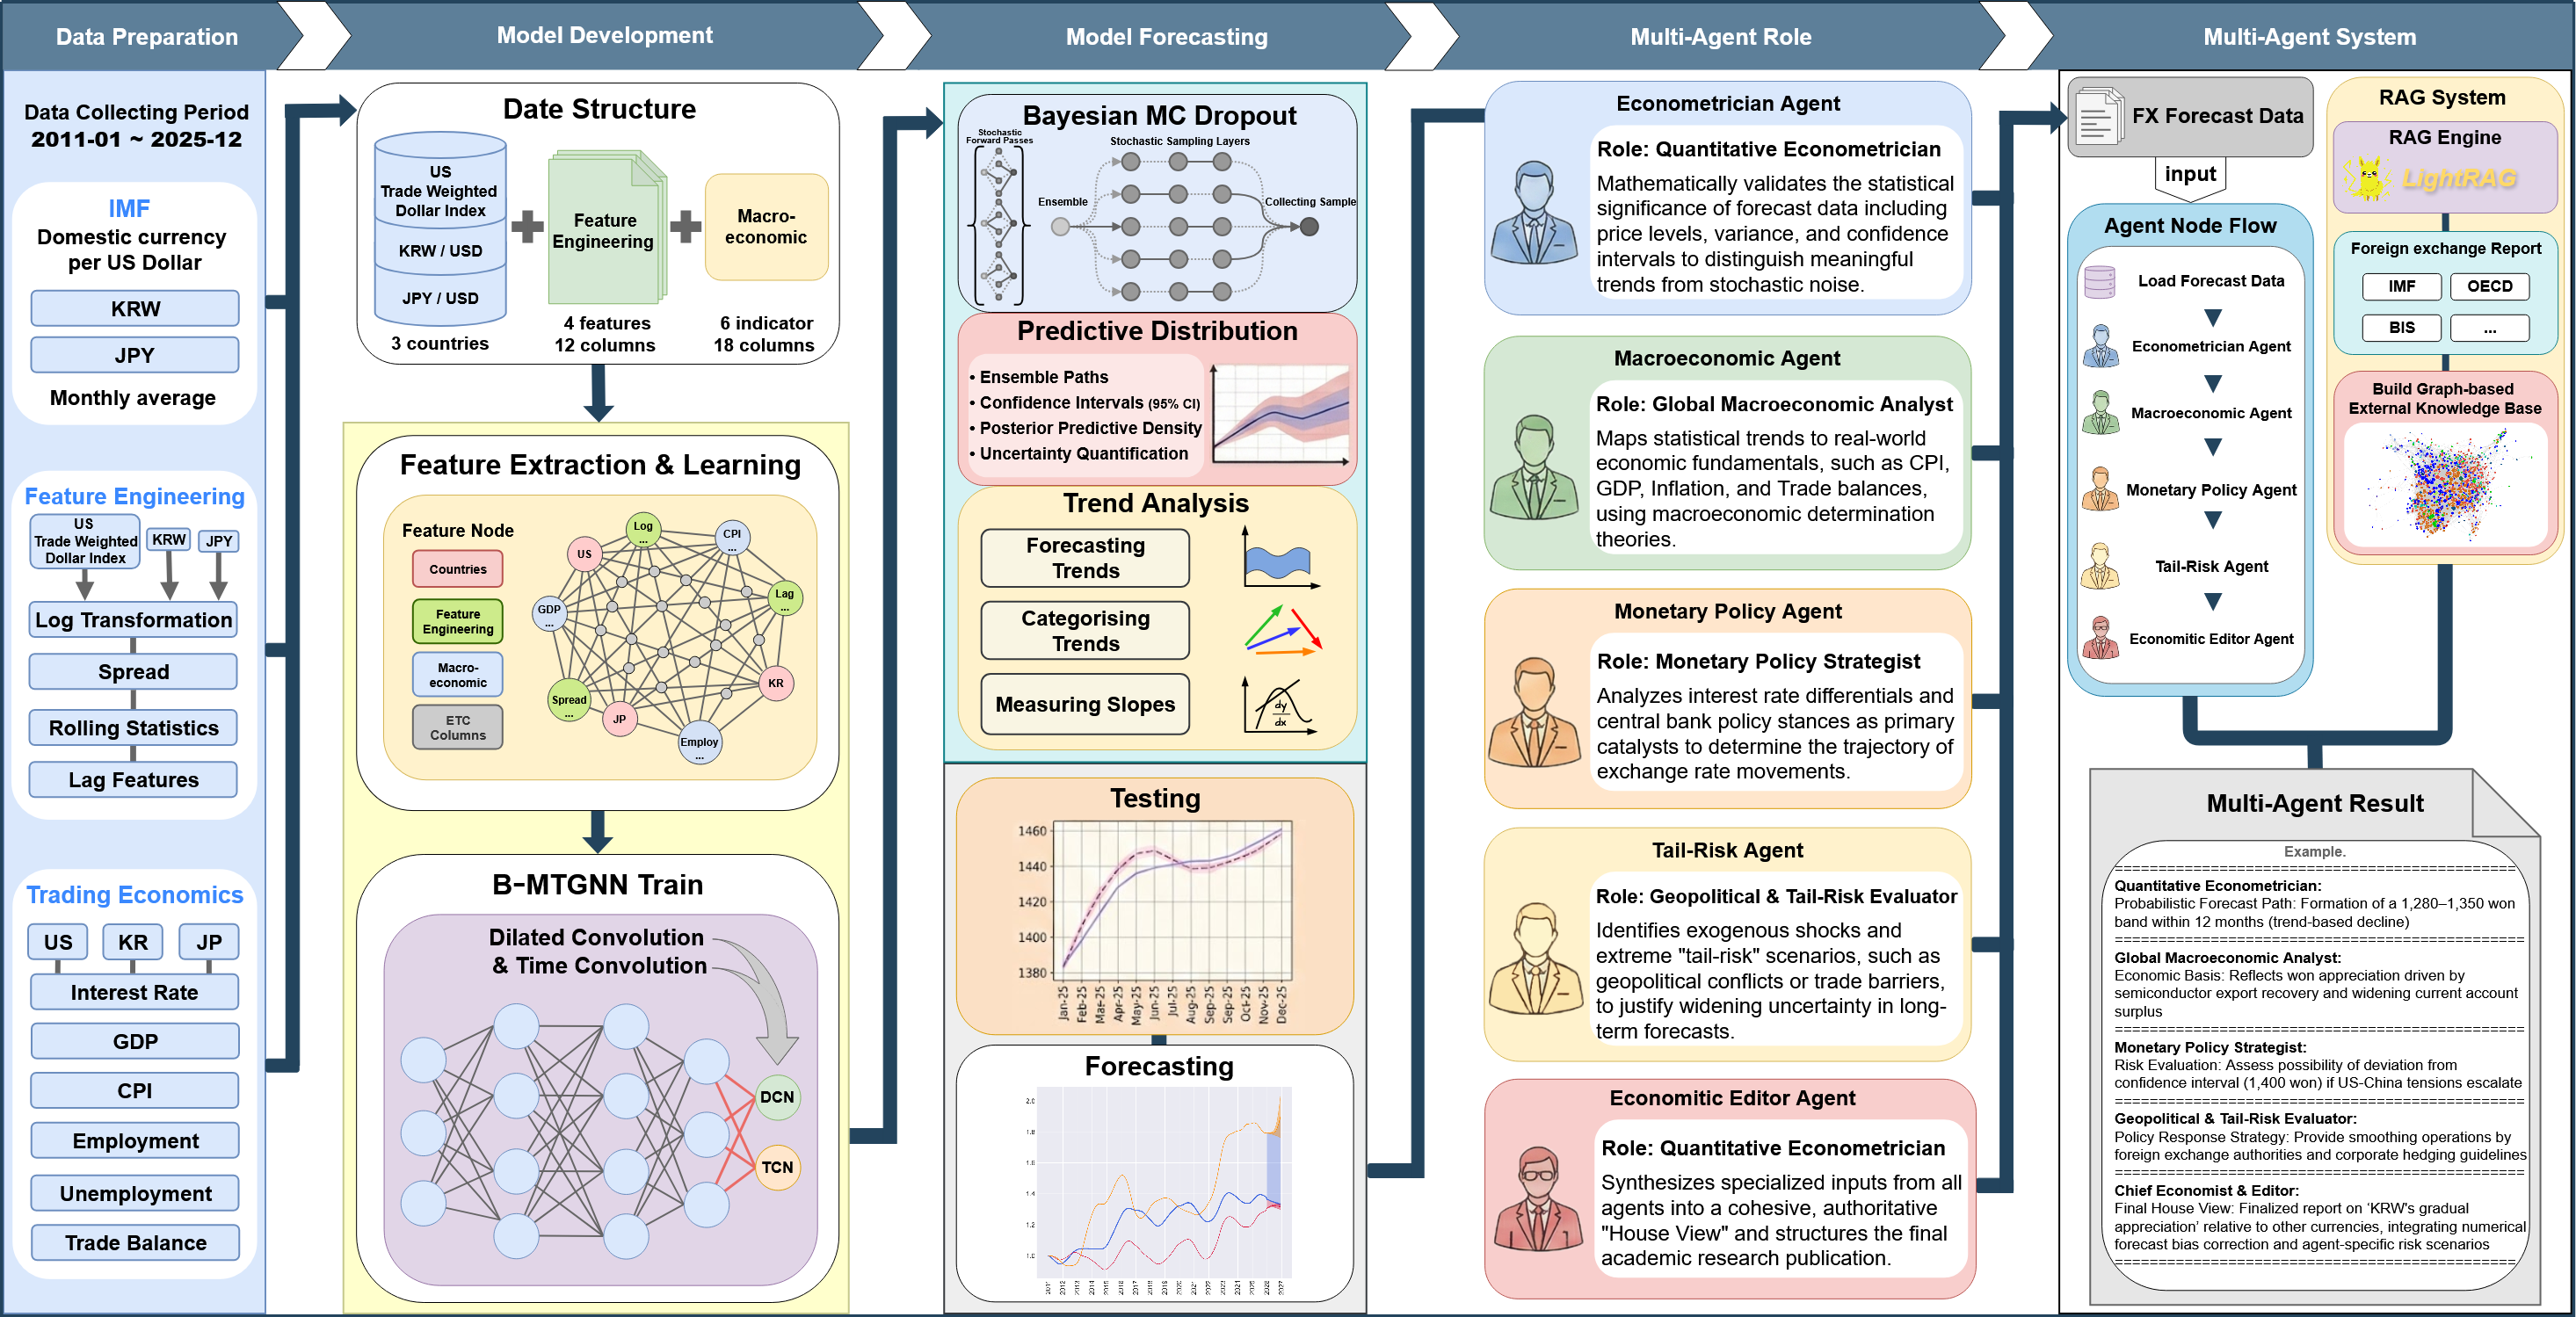
\includegraphics[width=\textwidth]{figure/fx_framework.drawio.png}}
\caption{국가 간 환율 변동 구조 예측을 위한 AI 프레임워크: 다변량 시계열 데이터, B-MTGNN 기반 예측, 추세–격차 분석, 멀티 에이전트 검증을 통합하여 전략적 외환 분석 결과 해석}
\label{fig:framework}
\end{figure*}

\subsection{입력 변수 및 정보 구성}
환율은 단일 요인으로 움직이지 않으며, 환율 자체의 변동 구조와 국가 간의 상호작용에 따라 서로 영향을 주며 함께 변한다. 이에 따라 본 연구는 각 국가 $i$에 대해 다음의 구성요소를 결합한다. 국가 $i$의 환율 관측을 $E_i(t)$라 할 때, 모델의 기초 입력이 되는 로그 수익률을 $Y_i(t)$로 정의한다.
% 기초입력이 로그 수익률?
\begin{equation}
Y_i(t)=\log E_i(t)-\log E_i(t-1)
\tag{2}
\end{equation}
본 연구에서는 딥러닝 모델의 학습 안정성을 위해 $Y_i(t)$를 환율 상태로 정의한다. 모델이 국가 간 단기 흐름과 함께 움직이는 패턴을 명시적으로 포착할 수 있도록, 특성 공학을 통한 입력 변수 가공으로 과거 수익률 값, 국가 간 수익률 격차, 그리고 롤링 상관계수를 파생 지표 $F_i(t)$ 집합으로 포함하였다. 이와 함께 국가 경제에 구조적 영향을 미치는 정책 금리, GDP, 소비자물가지수, 고용 지표, 실업률, 무역 수지 등의 주요 거시·금융 지표를 $M_i(t)$로 둔다. 최종적으로 국가 $i$의 시점 $t$ 입력 다변량 특징 벡터는 다음과 같이 수식화된다.
% Feature engineering 직접 언급
\begin{equation}
\mathbf{x}_i(t)=\big[\,Y_i(t),F_i(t),M_i(t)\,\big]
\tag{3}
\end{equation}

\subsection{국가 상호작용 그래프 구성}
국가 간 구조적 의존성을 명시적으로 반영하기 위해 가중 그래프를 정의한다.
\begin{equation}
G=(V,E,A)
\tag{4}
\end{equation}
여기서 $V=C$는 국가(통화) 노드 집합, $E\subseteq V\times V$는 국가 간 관계, $A\in\mathbb{R}^{N\times N}$는 가중 인접행렬이다. 엣지 $(c_i,c_j)$는 무역노출, 금융통합, 통화정책의 파급 효과, 지역 인접성, 환율 상관 기반 연동성 등으로 인해 $i$의 변화가 $j$에 영향을 줄 수 있음을 의미한다.
초기 인접행렬 $A$는 상관, 경제/지역 근접성, 잠재 의존 성분을 혼합해 구성할 수 있으며,
\begin{equation}
A_{ij}=\alpha A^{\mathrm{corr}}_{ij}+\beta A^{\mathrm{econ}}_{ij}+\gamma A^{\mathrm{latent}}_{ij}
\tag{5}
\end{equation}
처럼 가중 결합 형태로 나타낼 수 있다. 학습 과정에서 그래프 구조가 메시지 전달 과정 등을 통해 점진적으로 개선될 수 있다.

\subsection{B--MTGNN 예측}
시점 $t$에서 노드 특징 행렬을
\begin{equation}
X(t)\in\mathbb{R}^{N\times d}
\tag{6}
\end{equation}
로 두고, 각 행이 $\mathbf{x}_i(t)$에 대응한다. 관측 $\{X(1),\dots,X(T)\}$ 및 그래프 $G$가 주어졌을 때, 목적은 미래 환율 상태의 예측분포를 추정하는 것이다. % 말이 어색함.
\begin{equation}
p\!\left(\mathbf{Y}_{T+1:T+H}\mid \mathbf{X}_{1:T},G\right)
\tag{7}
\end{equation}

\paragraph{베이지안 불확실성 추정}
예측 결과의 불확실성을 측정하기 위해 몬테카를로 드롭아웃(Monte Carlo Dropout, MC Dropout) 기반 베이지안 추론을 사용한다. 예측 단계에서도 드롭아웃을 활성화한 상태에서 동일 입력에 대해 모델 예측을 반복 수행하여 확률적 예측 분포를 추정한다.

\begin{equation}
\hat{\mathbf{Y}}^{(s)}(T+h)=f_{\theta^{(s)}}\!\left(\mathbf{X}_{1:T},G\right),\quad s=1,\dots,S
\tag{8}
\end{equation}
이로부터 예측 평균과 분산을 수식 9와 같이 계산한다. % 다음과 -> 수식 9와
\begin{equation}
\begin{aligned}
\mu_{T+h} &= \frac{1}{S}\sum_{s=1}^{S}\hat{\mathbf{Y}}^{(s)}(T+h),\\
\sigma^2_{\mathrm{MC},T+h} &= \frac{1}{S-1}\sum_{s=1}^{S}\left(\hat{\mathbf{Y}}^{(s)}(T+h)-\mu_{T+h}\right)^2
\end{aligned}
\tag{9}
\end{equation}
구현 단계에서는 MC Dropout 반복 추론을 통해 얻은 분포의 분위수를 기반으로 예측구간을 산출하며, 예측의 불확실성을 나타내는 95\% 신뢰구간을 산출한다.

\paragraph{국가 간 환율 격차 정의}
국가 $i$와 $j$의 상대적 환율 격차를 예측 평균 기반으로 정의한다.
\begin{equation}
\mathrm{Gap}_{i,j}(T+h)=\mathbb{E}\!\left[Y_i(T+h)\right]-\mathbb{E}\!\left[Y_j(T+h)\right]
\tag{10}
\end{equation}
$\mathrm{Gap}_{i,j}(T+h)$는 $h$시점에서 통화 $i$ 대비 통화 $j$ 환율 변화량의 상대적 우위와 방향성을 나타내며, 값이 양수면 $i$의 상대적 강세, 음수면 상대적 약세를 의미한다. 분위수 구간을 함께 보고하면 격차 추정의 불확실성과 부호의 견고성까지 해석할 수 있다.
본 연구에서 각 환율 상태 $Y_i$는 기준점(1.0)을 바탕으로 정규화된 수치로 산출되며, 이에 따라 도출된 격차 역시 서로 다른 단위의 통화 간에도 직접 비교가 가능한 정규화된 수치의 절대적 차이를 의미한다.

\subsection{멀티 에이전트 기반 검증}
앞선 B--MTGNN 모델은 시계열 데이터에 내재하고 있는 패턴과 상호작용을 학습하여 환율을 정량적으로 예측하면서 통계적 불확실성까지 산출하게 된다. 그러나 시계열 데이터 기반의 예측만으로는 외환 시장을 둘러싼 복잡하고 상호 연결된 거시경제 변화, 통화정책의 구조 변경 등 모델이 학습하기 어려운 요인들을 시장에 반영하는 데 근본적인 한계가 존재한다. 이를 보완하기 위해 본 연구는 검색 증강 생성(Retrieval-Augmented Generation, RAG)를 통해 금융 기반의 외부 지식 도메인을 결합한 LangGraph 프레임워크 기반의 멀티 에이전트 시스템을 도입하여 환율 예측 결과의 설명 가능성과 판단 근거를 강화한다~\cite{Isufaj2025,Yu2023Temporal}. 본 시스템에서 분석을 수행하는 에이전트별 구체적 역할은 표~\ref{tab:agents}과 같이 정의된다.

\begin{table}[ht]
\centering
\caption{에이전트 역할 정의}
\label{tab:agents}
\small
\setlength{\tabcolsep}{3pt}
\begin{tabular}{p{0.35\linewidth}p{0.6\linewidth}}
\toprule
역할 & 내용 \\
\midrule
계량경제 분석가 & 모델 예측 결과의 통계적 유의성 및 분산 검증\\ \addlinespace[3pt]
거시경제 분석가 & 경제 성장률, 인플레이션 등 거시경제 요인 분석\\ \addlinespace[3pt]
통화정책 전략가 & 중앙은행 금리, 가계부채 등 통화기조가 환율 변화에 미치는 영향 모델링\\ \addlinespace[3pt]
비정형 위험 분석가 & 국가별 경제 변화와 같은 모델이 포착하지 못하는 비정형 요소 분석 및 평가\\ \addlinespace[3pt]
종합 분석가 & 에이전트의 결과를 종합하여 금융 보고서 형태의 정량/정성적 결과 도출\\
\bottomrule
\end{tabular}
\end{table}

\paragraph{멀티 에이전트의 그래프 기반 상태 머신과 RAG 엔진}
해당 시스템은 단일 LLM에 모든 과정을 의존하는 기존의 프롬프팅 방식과 달리, 그래프 기반의 상태 머신(State Machine) 구조를 통해 분석 과정을 세분화한다~\cite{Wu2024LangGraph}. 긴 컨텍스트에서 중간 정보를 망각하는 문제가 보고된 바 있으며\cite{Liu2024Lost}, 본 연구에서는 각 단계에서 도출된 전문 에이전트의 분석 결과는 상태 저장소에 저장되며, 다음 노드의 입력 컨텍스트로 전달된다. 이러한 그래프 기반 상태 저장소 설계는 각 에이전트의 추론 정보를 누적 저장함으로써 망각 현상을 방지한다~\cite{Packer2023MemGPT}. 또한 현재 시스템에서 사용된 모델은 Mistral AI의 Ministral-3:8b으로~\cite{Liu2026Ministral}, 이러한 구조는 상대적으로 파라미터 수가 적은 SLM이 개별 추론 단계에서 겪을 수 있는 인지적 부하를 효과적으로 분산시킨다. 결과적으로 제한된 처리 자원 내에서도 손실 없는 정보 처리를 가능하게 하며, 경제적이면서도 높은 일관성을 갖춘 추론 결과를 확보하는 데 기여한다.

본 시스템은 거시경제 지표와 환율 변동 간의 인과관계를 정밀하게 검증하기 위해 LightRAG를 RAG 엔진으로 채택하여 외부 도메인 지식을 통합하였다~\cite{Guo2024LightRAG}. 기존의 단순 벡터 검색 방식과 달리, 제안하는 방식은 IMF, OECD, BIS 등 실제 경제 보고서에서 추출한 내용과 이들 사이의 인과 관계를 지식 그래프 형태로 구조화하여 저장한다. 이때 추출된 인과 관계 정보는 고차원 벡터 공간 내에서 단순 키워드 매칭의 한계를 넘어선 의미론적 연관성 검색을 지원한다~\cite{Edge2024GraphRAG}. 이러한 설계는 각 에이전트의 추론 결과가 외부 지식 베이스와 실시간으로 동기화되도록 한다. 결과적으로 에이전트는 단편적인 텍스트 매칭을 넘어, 고차원적 맥락에 기반한 경제적 기초 요인 분석이 가능한 지식 체계를 갖추게 된다.

\paragraph{에이전트 추론 및 상태 전이 구성}
본 연구의 다중 에이전트 시스템은 다중 에이전트 간 선형적 상태 전이 구조를 가진다. 이를 정형화하기 위해 예측의 정성적 해석을 수행하는 $K$개의 전문 에이전트의 집합을 $\mathcal{A} = \{a_1, a_2, \dots, a_k\}$라 정의한다. (표~\ref{tab:agents}에 따라 본 연구에서는 $K=5$)

관측 시점 $T$에서 시스템의 초기 상태(State) $s_0$는 3.4절에서 정의된 B--MTGNN 모델의 산출물과 금융 경제 기반 컨텍스트의 결합으로 정의된다. 즉, 예측 구간 $H$에 대한 예측 평균 시퀀스 $\boldsymbol{\mu}_{T+1:T+H}$ (수식 9 참조), MC dropout을 통한 베이지안 예측 확률 분포 $\boldsymbol{\sigma}^2_{\mathrm{MC}, T+1:T+H}$, 그리고 롤링 윈도우(Rolling Window)의 거시금융 입력 특징 벡터 $\mathbf{X}_{T}$를 초기 상태로 구성한다.
\setcounter{equation}{10}
\begin{equation}
s_0 = \big\langle \boldsymbol{\mu}_{T+1:T+H}, \; \boldsymbol{\sigma}^2_{\mathrm{MC}, T+1:T+H}, \; \mathbf{X}_{T} \big\rangle
\end{equation}
여기서 산출된 정량적 특징 벡터 $s_0$는 에이전트가 이해할 수 있는 자연어 기반의 컨텍스트 형태로 변환되어 노드에 전달된다. 이후 각 에이전트 수행 단계 $k \in \{1, \dots, K\}$에서 에이전트 $a_k$는 이전 단계의 추론 상태 $s_{k-1}$과 LightRAG 엔진을 통해 외부 지식 그래프에서 검색한 도메인 특화 컨텍스트 $\mathcal{R}_k(s_{k-1})$를 입력으로 받아들여, 해당 도메인 특화 해석 근거를 담은 추론 결과 $e_k$를 생성한다.
\begin{equation}
e_k = a_k\!\left(s_{k-1}, \, \mathcal{R}_k(s_{k-1})\right)
\end{equation}
여기서 $\mathcal{R}_k(\cdot)$는 $k$번째 에이전트의 역할 프롬프트에 연동된 RAG 검색 함수를 의미한다. 이때 도출된 분석 결과 $e_k$는 단순 출력물로 그치지 않고 다음 노드로 전이되며, 동시에 RAG 메모리 공간 $\mathcal{M}$에 임베딩된다.
\begin{equation}
\begin{aligned}
s_k &= s_{k-1} \oplus e_k \\
\mathcal{M}^{(k)} &= \mathcal{M}^{(k-1)} \cup \text{Embed}(e_k)
\end{aligned}
\end{equation}
위 식의 $\oplus$는 모델의 예측 수치와 텍스트 형태 추론 결과의 의미론적 결합(Semantic concatenation)을 표현한다.
결과적으로 파이프라인의 종점인 $K$번째 에이전트는 누적된 전체 분석 결과를 종합하여, 다차원적(정량·거시·정책·리스크)으로 검증된 최종 환율 전망 및 동향 분석 $\mathcal{S}_{\text{final}}$을 출력한다.
\begin{equation}
\mathcal{S}_{\text{final}} = a_K(s_{K-1}, \mathcal{R}_K)
\end{equation}
이러한 마르코프 연쇄(Markov chain) 구조의 선형적 수식화는, 앞서 언급한 바와 같이 SLM의 컨텍스트 길이를 넘지 않으면서 모델의 추론 심도를 개선함으로써 예측 모델의 설명 불가능한 복잡한 환율과 거시경제의 관계를 학술적으로 입증한다.


\section{실험 결과}
\titlespacing*{\subsection}{0pt}{1.0em}{0.3em}
\titlespacing*{\paragraph}{0pt}{1.0em}{0.3em}

본 절에서는 국가 간 상호의존성과 높은 시계열 변동성을 보이는 외환 시장 환경에 B--MTGNN 모델을 적용하여 환율 간 구조적 관계를 학습하고 환율 예측을 수행한 실증 분석 결과를 제시한다.

\subsection{실험 환경}
본 연구는 2011년 1월--2025년 12월(180개월)의 월별 데이터를 사용하였으며, 학습 구간은 2011년 1월--2023년 12월(156개월), 검증 구간은 2024년 1월--12월(12개월), 평가 구간은 2025년 1월--12월(12개월)로 분할하였다. 분석 대상 통화는 미국(US Trade Weighted Dollar Index), 한국(KRW), 일본(JPY)의 세 국가로 설정하였다. 모델 입력은 총 33개 환율, 특성공학 그리고 환율 및 거시경제 변수로 구성된 월별 다변량 시계열 데이터이며, 이는 3개의 환율 변수와 12개의 특성 공학(Feature Engineering) 변수 그리고 18개의 거시경제 변수로 이루어진다. 특성 공학 변수에는 각 통화의 수익률, 수익률의 시차 변수, 통화 간 수익률 차이, 그리고 통화 간 상관계수와 같은 시장 기반 파생 변수가 포함된다. 거시경제 변수는 각 국가의 거시경제 환경을 반영하기 위해 금리, 국내총생산(GDP), 소비자물가지수(CPI), 고용, 실업률, 무역수지로 여섯 가지 지표를 미국, 한국, 일본에 대해 각각 수집하여 총 18개 변수로 구성하였다. 국가별 시계열 데이터는 서로 다른 휴일제, 거시경제 지표 발표일 등으로 인한 시차를 가질 수 있다. 본 연구에서는 모든 시계열을 월별 기준으로 수집하고, 관측치가 존재하지 않는 구간에 대해서는 직전 관측치 기반 데이터를 대체하는 전진 채움 기법을 적용하여 데이터의 연속성을 확보하였다. 또한, 관측되지 않는 결측치는 모델 학습 시 해당 입력값의 영향을 배제하는 마스킹 기법을 통해 처리하여, 결측치 자체가 예측에 왜곡된 영향을 미치는 것을 방지한다. 이러한 변수 구성은 통화 가치에 영향을 미치는 실물경제 및 금융 요인을 동시에 반영하기 위한 것이다.
베이지안 그래프 신경망의 주요 하이퍼파라미터는 학습률 0.00015, Dropout 0.02, 은닉 차원 256, 학습 에폭 180으로 구성되었다. 

\subsection{실험 결과}
테스트 성능 평가는 Root Relative Squared Error(RRSE)를 기준으로 평가되었으며, 평가 구간에서의 예측 결과 시각화와 통계적 검증을 통해 모델의 성능을 보수적으로 검증하였다.

\paragraph{예측 모델 성능 평가}
표~\ref{tab:forecast_2026}는 평가 구간인 2025년 1월부터 2025년 12월까지에 대한 모델 예측 성능을 요약한 것이다. 일본 엔화(JPY)가 0.2832로 가장 낮은 RRSE를 기록하여 세 통화 중 가장 높은 예측 정확도를 보였으며, 한국 원화(KRW)는 0.3374, 미국 달러 지수(US Trade Weighted Dollar Index)는 0.5159로 나타났다. 다음으로 그림~\ref{fig:testing_fx_all}는 평가구간의 월별 환율 예측 결과를 시각적으로 나타낸 것이다. 각 그래프에서 파란색 실선은 실제 환율 추세, 보라색 점선은 모델이 예측한 값, 그리고 분홍색 음영 영역은 95\% 신뢰 구간을 의미한다. 미국 달러 지수의 경우 상반기에는 상승 추세가 나타났다가 하반기로 갈수록 점진적으로 하락하는 패턴이 관찰된다. 한국 원화 환율의 경우 연초 이후 상승 흐름이 나타난 뒤 중반 이후 비교적 완만한 상승세가 이어지는 패턴을 보인다. 일본 엔화 환율의 경우 상반기에는 하락 추세가 나타나고 이후 완만한 안정 구간이 형성되는 특징을 보인다. 모델은 이러한 장기적인 상승 추세를 비교적 정확하게 포착하고 있으며, 일부 시점에서 실제값과 예측값 사이의 편차가 존재하지만, 전반적인 추세 방향은 일관되게 유지되는 것을 확인할 수 있다. 그리고 하락 후 안정화되는 흐름을 비교적 잘 반영하고 있으며, 실제 환율 값이 대부분 신뢰 구간 내에 포함되어 예측 신뢰성이 유지되었다.

\begin{figure*}[!t]
\centering
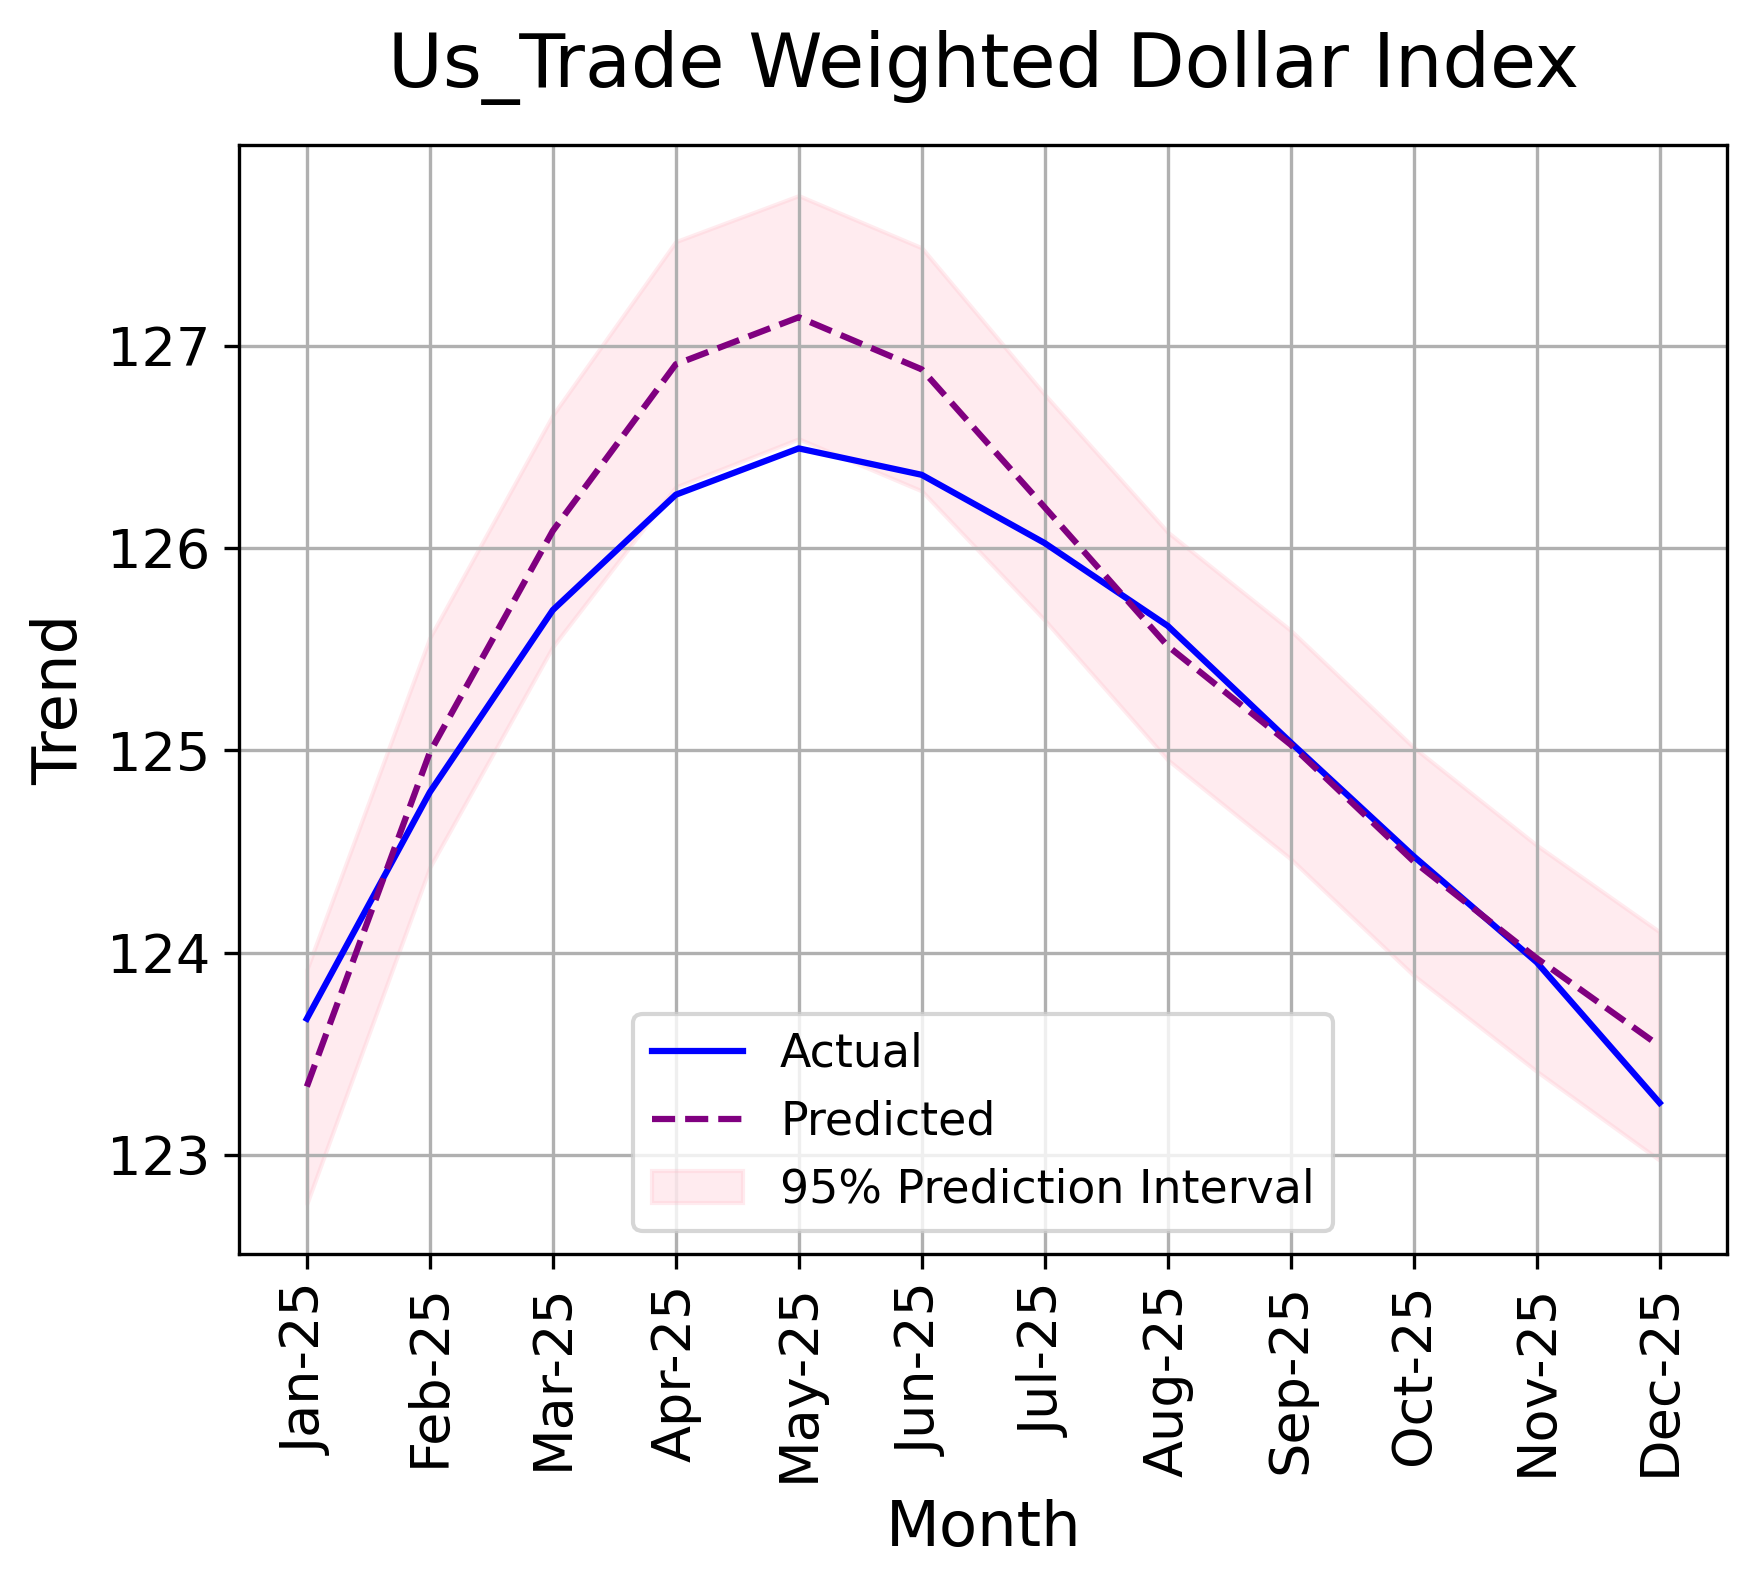
\includegraphics[width=0.32\textwidth]{figure/Us_Trade Weighted Dollar Index_Testing.png}
\hfill
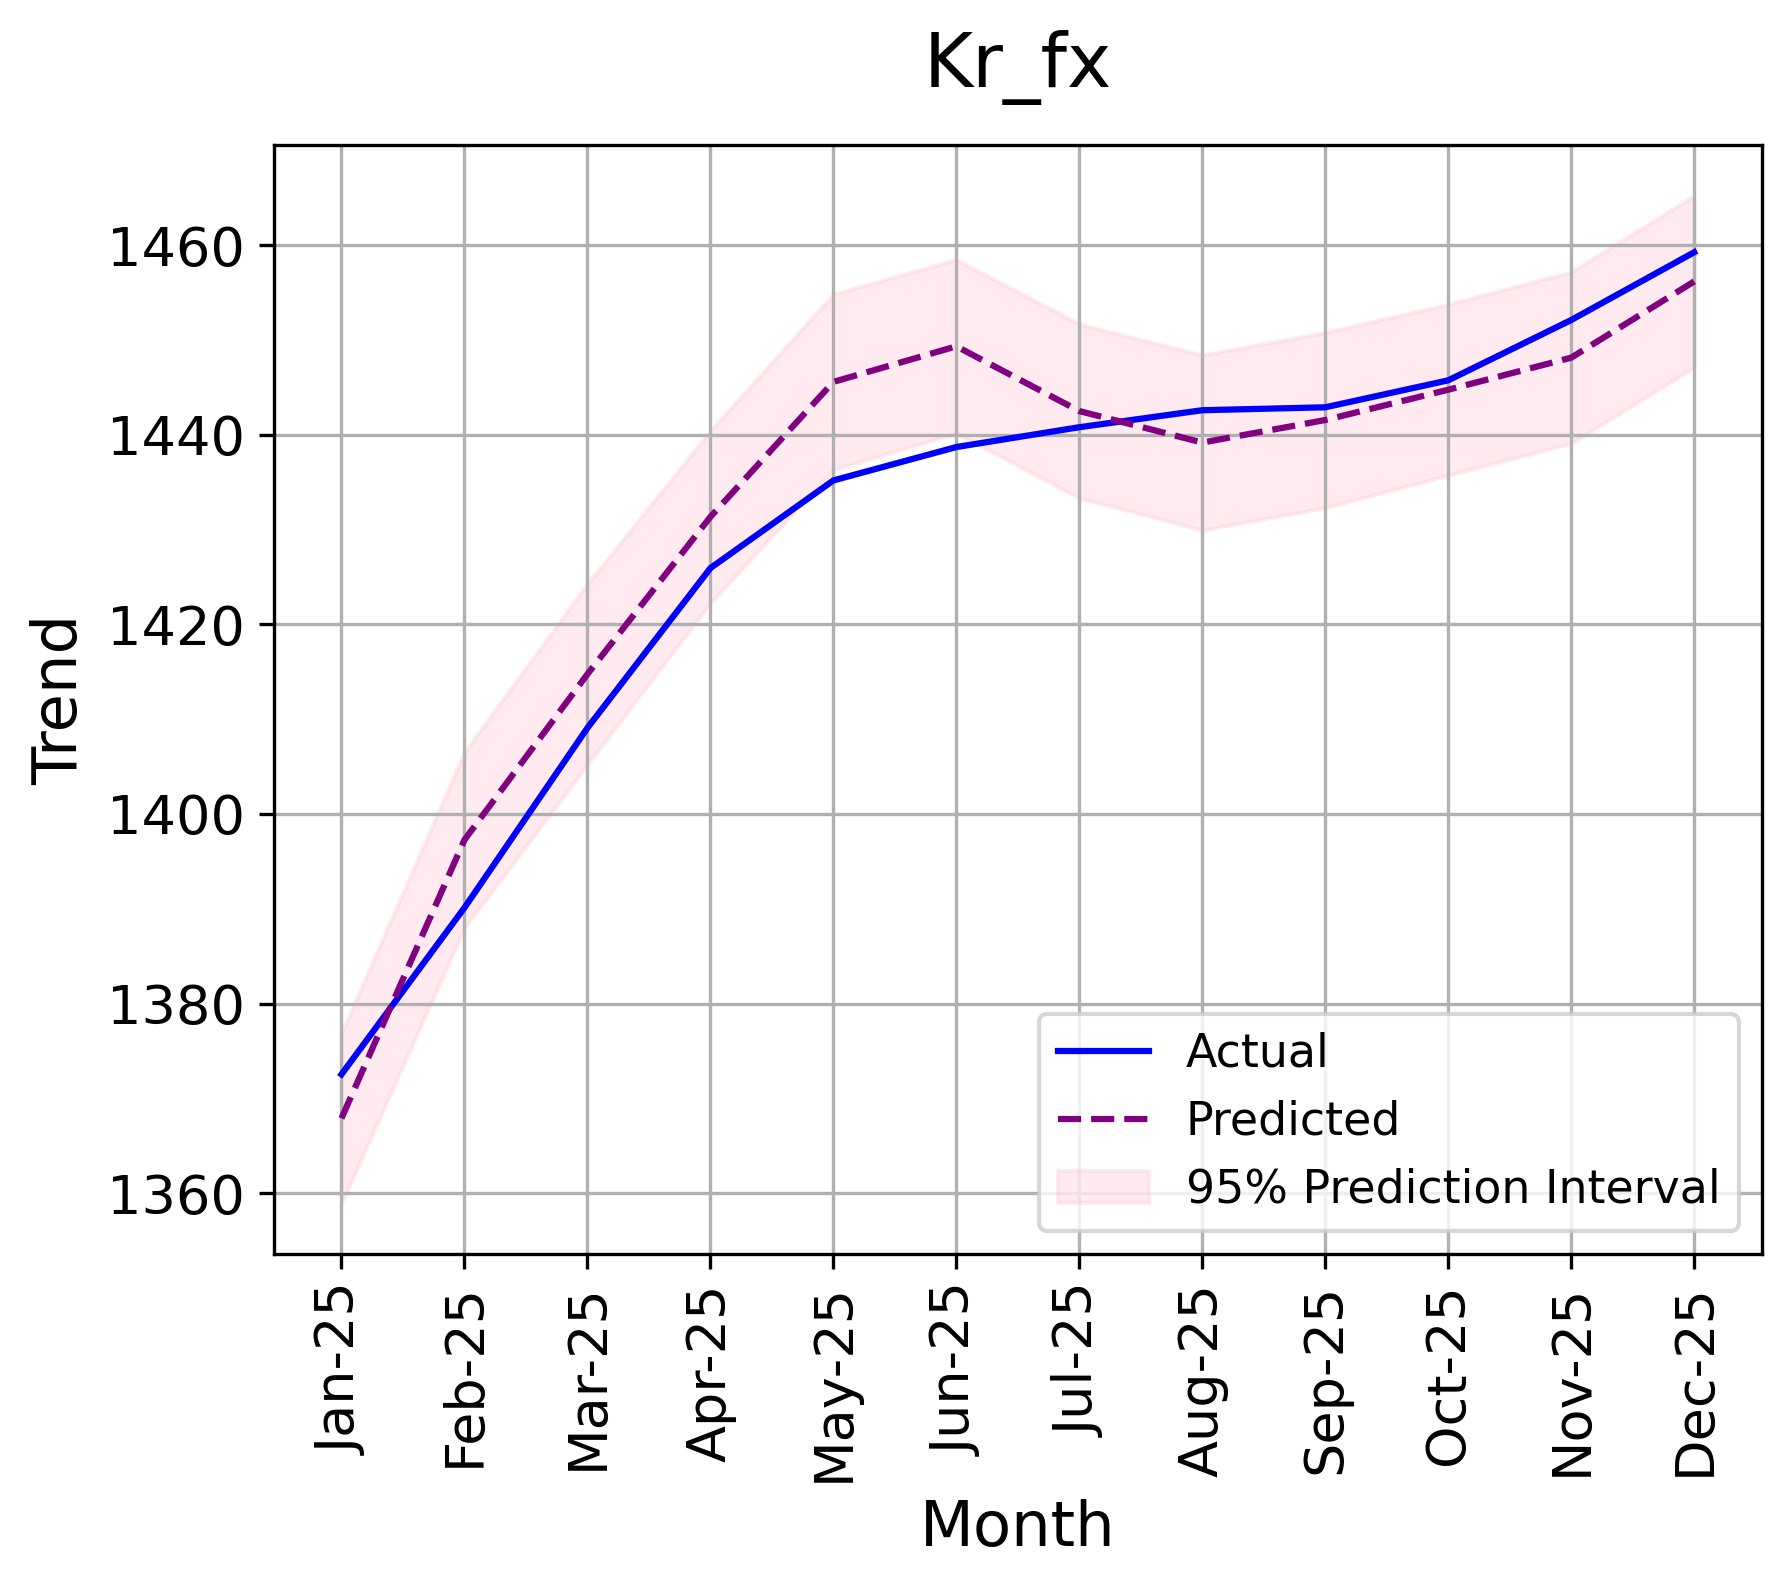
\includegraphics[width=0.32\textwidth]{figure/Kr_fx_Testing.png}
\hfill
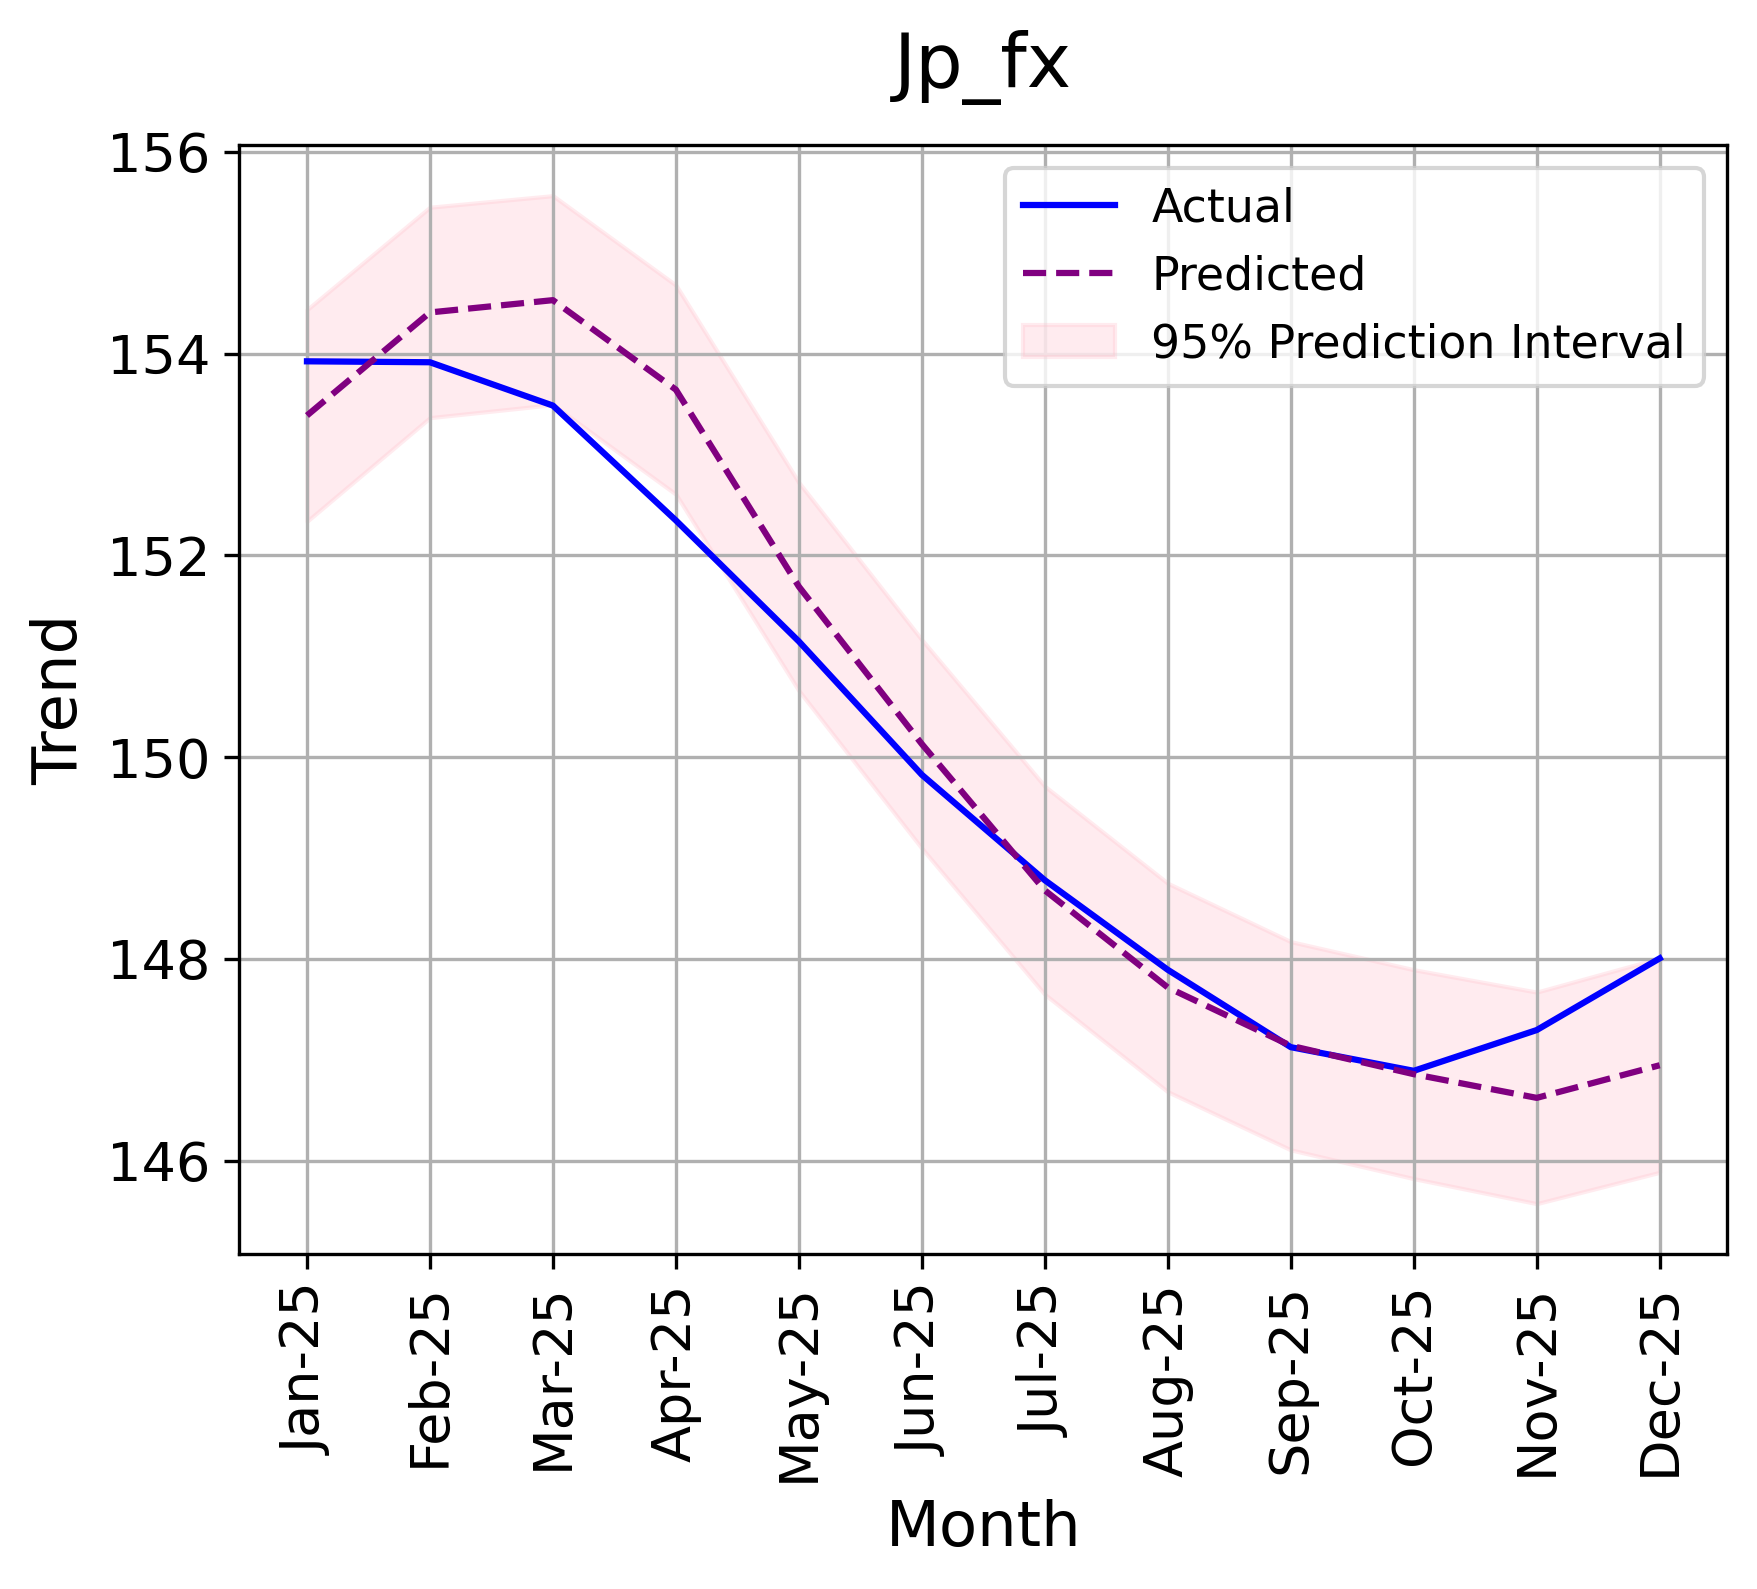
\includegraphics[width=0.32\textwidth]{figure/Jp_fx_Testing.png}
\caption{B--MTGNN 평가구간 성능 검증(좌 : US, 중 : KR, 우 : JP)}
\label{fig:testing_fx_all}
\end{figure*}

\paragraph{2026년 전망 및 결과}
2025년 12월까지의 관측값을 모델 학습으로 활용하여 2026년 1월--12월에 대한 환율 전망을 예측하였다. 표~\ref{tab:forecast_2026}는 MC dropout의 반복 횟수를 20회로 확대하여 생성한 베이지안 예측을 요약한 결과이며, 예측 평균과 95\% 신뢰 구간을 제시한다. 그림~\ref{fig:forecast_2026_normalized}에서도 확인할 수 있듯이, 국가 간 환율 경로는 예측 구간에 따라 국가 조합별로 상이한 변동 구조 패턴이 관측되었다. 2026년 말 기준 예측값을 살펴보면 미국 달러 지수는 약 121--122 수준으로 예측되었으며, 예측 구간은 약 117.90--118.99 범위로 나타났다. 일본 엔화는 약 153 수준으로 예측되었으며, 예측 구간은 약 159.44--207.44 범위로 추정되었다. 한국 원화 환율은 약 1,470--1,480원 수준으로 예측되었으며, 예측 구간은 약 1,457.29--1,490.76 범위로 나타났다. 특히 일본의 경우, 예측 구간 진입과 동시에 급격히 상승하며 신뢰구간의 폭 또한 비약적으로 확대되는 패턴이 관측되었다. 반면, 미국은 소폭 하락하며 수렴하는 양상을 보였고, 한국은 좁은 신뢰구간을 유지하며 상대적으로 안정적인 경로를 형성하였다.

\begin{figure*}[!ht]
\centering
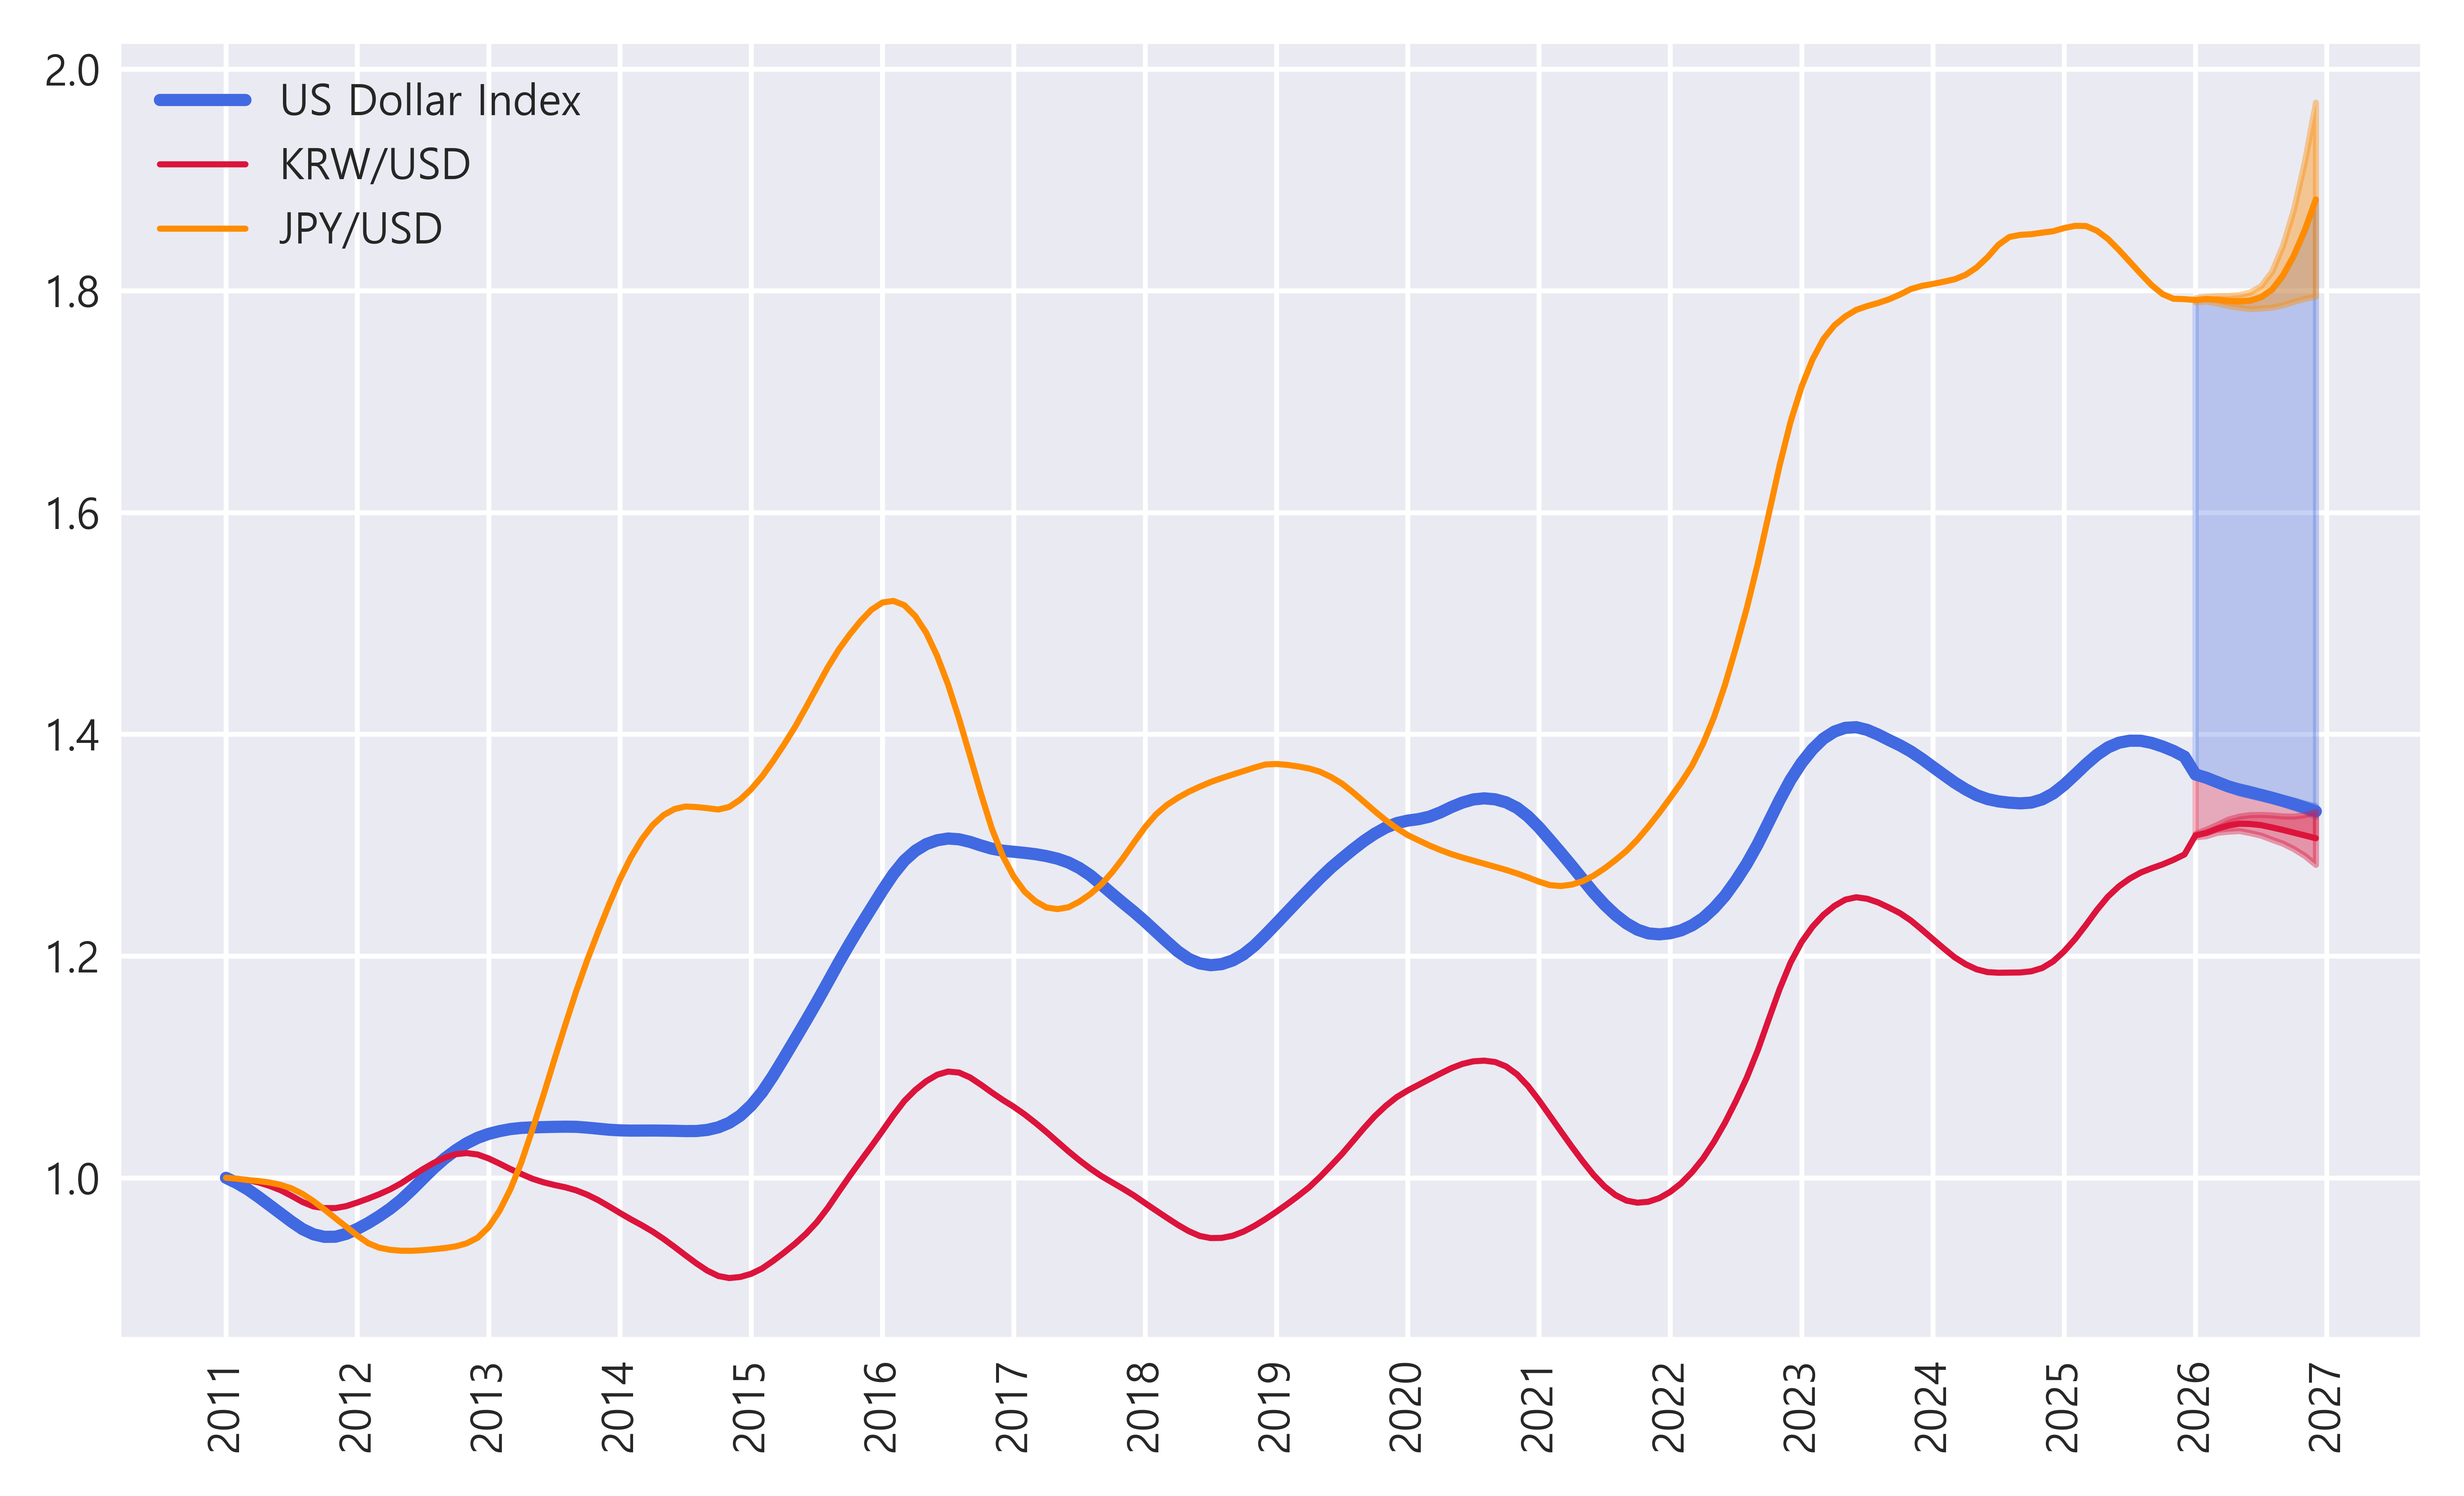
\includegraphics[width=\textwidth]{figure/Multi-Country Forecast Height Adjustment.png}
\caption{2026년 다중 통화 예측 경로(정규화). US Dollar Index와 KRW/USD 및 JPY/USD의 트렌드 예측 결과를 제시한다. 트렌드 플롯의 기간은 2011년 1월부터 2026년 12월까지이며, 이 중 2026년 1월부터 2026년 12월까지는 B--MTGNN 모델을 활용해 예측되었다. 환율 격차(Gap)는 해당 국가 환율 곡선과 동일한 색으로 강조되어 시각화되었다. 각 트렌드 예측에 대해서는 95\% 신뢰 구간이 함께 제시되어 있다. 각 환율 예측은 normalised 된 값이고 1.0은 정규화 기준점을 의미한다}
\label{fig:forecast_2026_normalized}
\end{figure*}

\begin{table}[t]
\centering
\caption{평가 구간 성능 및 예측 구간 요약}
\label{tab:forecast_2026}
\small
\setlength{\tabcolsep}{4pt}
\begin{tabular}{lccc}
\toprule
국가 & 성능검증$^{*}$ & 95\% 하한 & 95\% 상한 \\
\midrule
US (TWDI) & 0.5159 & 117.90 & 118.99 \\
JP (JPY)  & 0.2832 & 159.32 & 207.45 \\
KR (KRW)  & 0.3374 & 1457.29 & 1490.77 \\
\bottomrule
\multicolumn{4}{l}{\footnotesize $^{*}$성능검증평가: RRSE (Root Relative Squared Error)}
\end{tabular}
\end{table}

\paragraph{국가 간 예측 패턴 비교}
표~\ref{tab:gap_2026}은 2026년 예측된 환율 경로를 기반으로 국가 간 평균 수준 격차를 비교한 결과를 나타낸다. 각 값은 2026년 12개월 예측값을 평균하여 계산한 연간 평균 환율 차이로 정의된다. 분석 결과 일본--한국 조합이 0.637로 가장 큰 평균 격차를 보였으며, 일본--미국 조합은 0.61로 그다음으로 나타났다. 반면 미국--한국 조합은 0.026으로 상대적으로 작은 차이를 보였다. 이러한 결과는 세 국가 환율이 동일한 방향으로 움직이기보다는 국가별로 서로 다른 변동 경로와 조정 속도를 보일 가능성을 시사한다.

\begin{table}[t]
\centering
\caption{국가 간 상대적 환율 격차}
\label{tab:gap_2026}
\small
\setlength{\tabcolsep}{3pt}
\begin{tabular}{lc}
\toprule
국가 조합 & 평균 환율 격차 \\
\midrule
US--KR & 0.026 \\
JP--US & 0.610 \\
JP--KR & 0.637 \\
\bottomrule
\end{tabular}
\end{table}
\begin{figure}[!t]
\centering
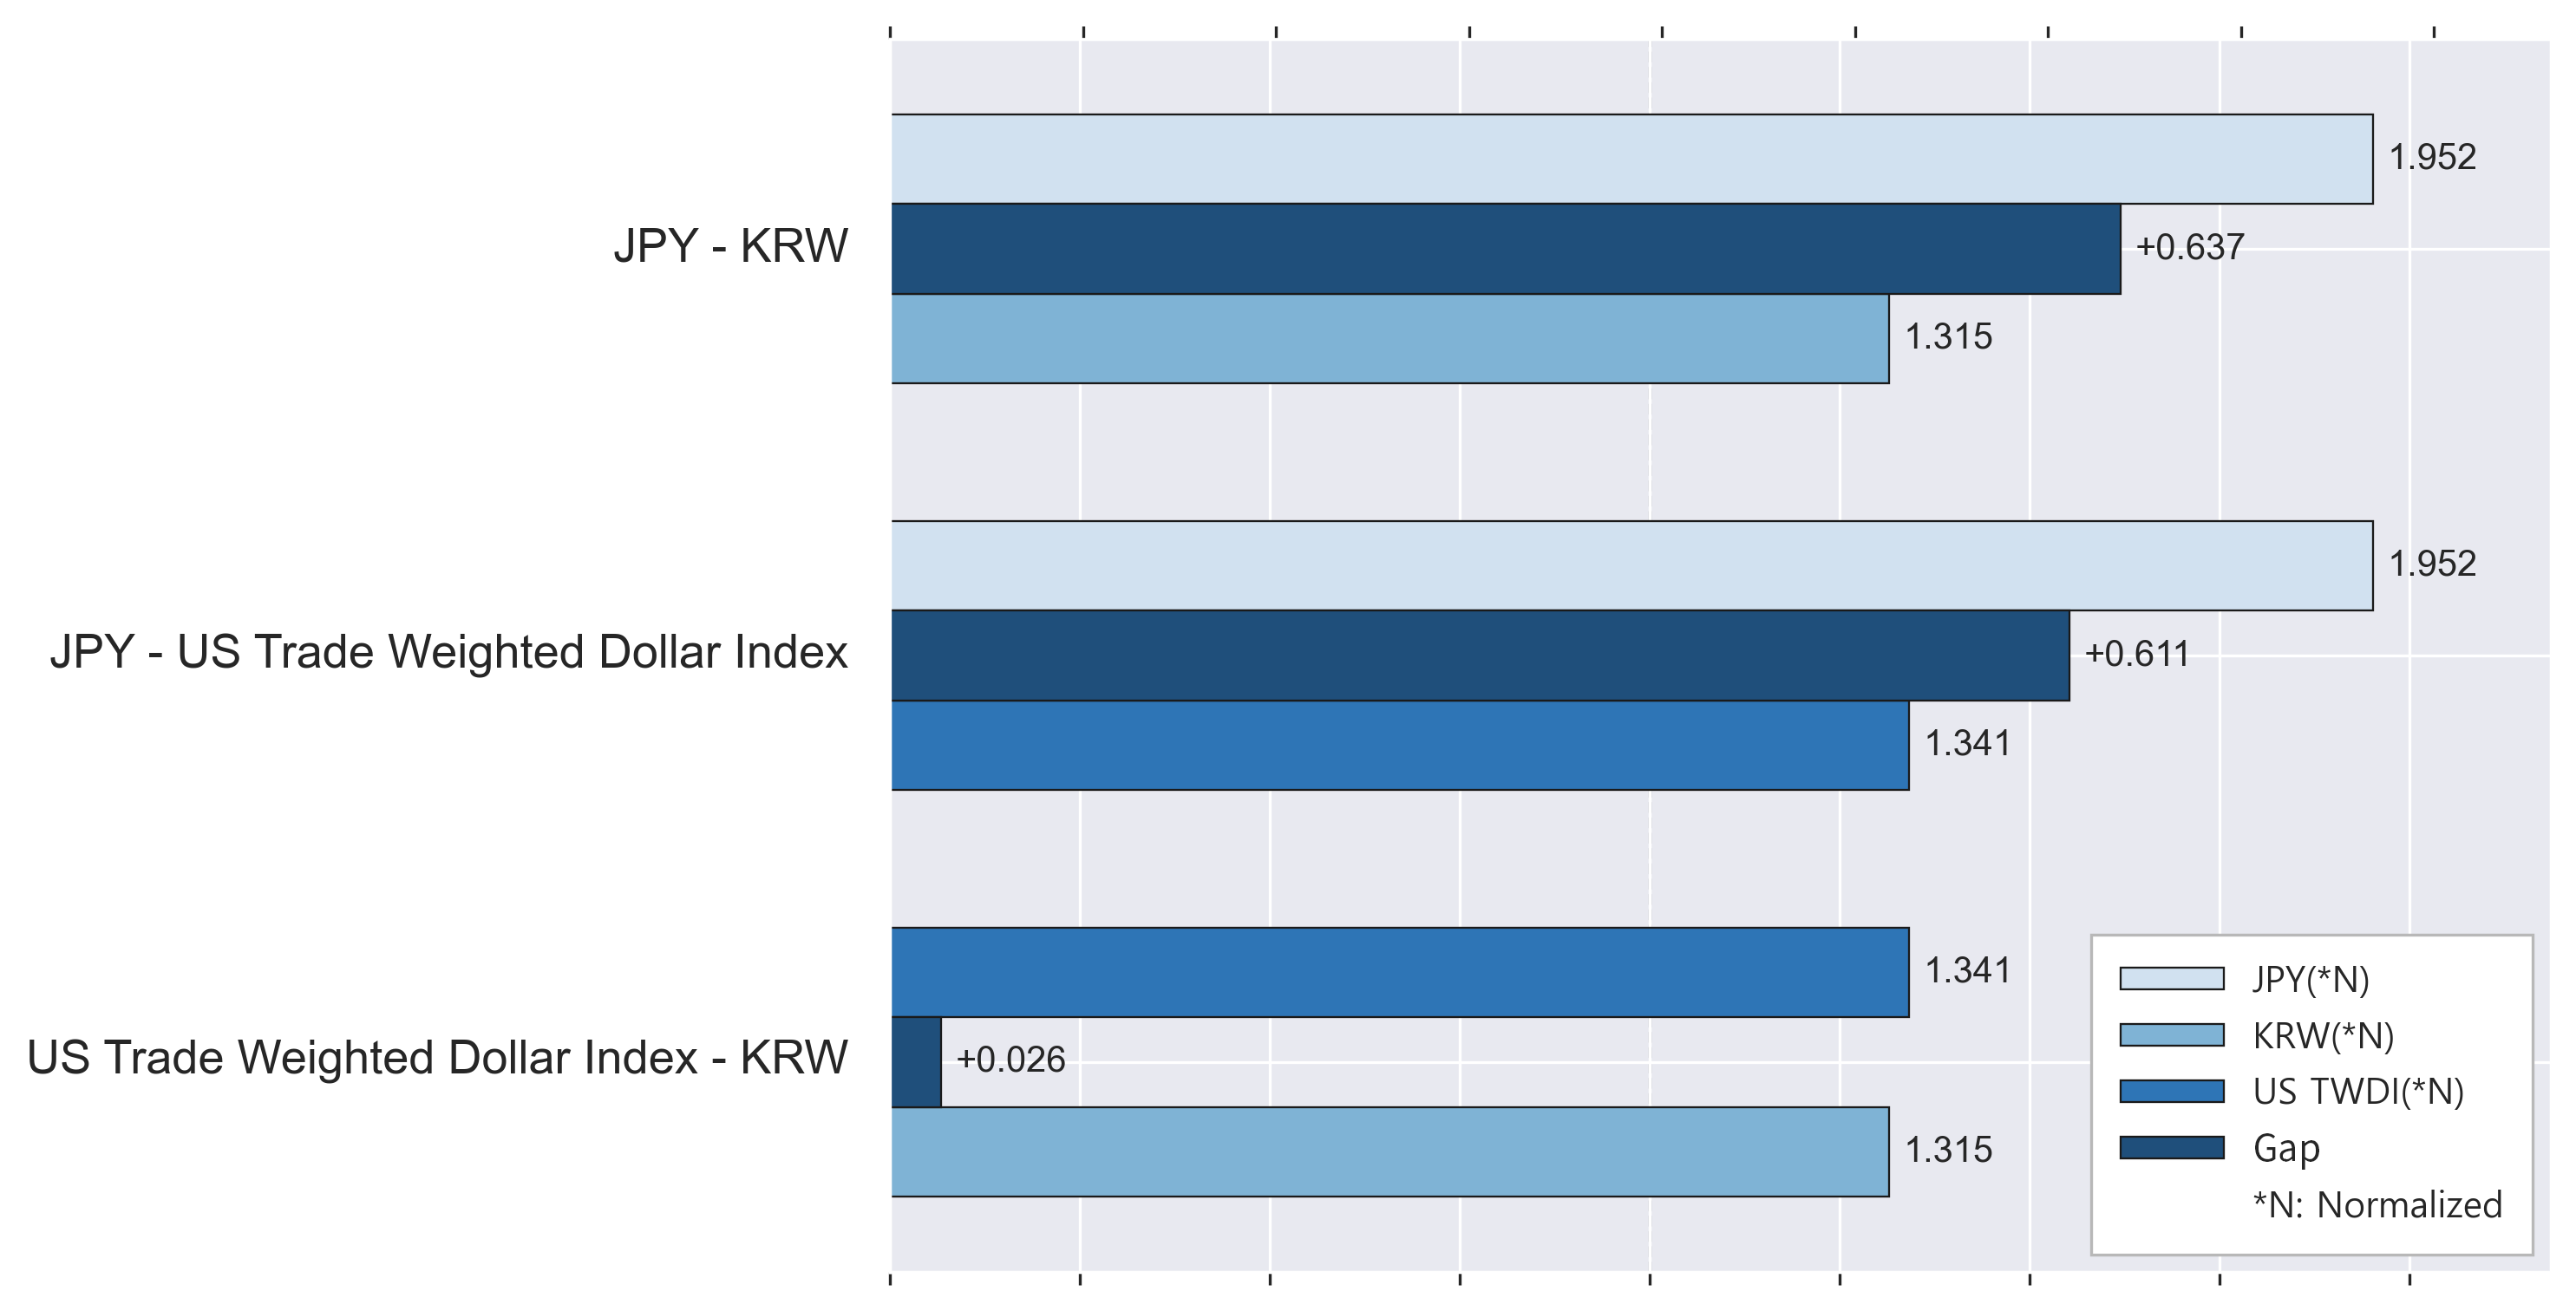
\includegraphics[width=\columnwidth]{figure/normalized_gap_bar_final.png}
\caption{국가 간 환율 격차($\mathrm{Gap}_{i,j}$) 비교}
\label{fig:normalized_gap_discussion}
\end{figure}

\paragraph{예측 모델 성능 연구 결과}
종합적으로 보았을 때, 제안한 B-MTGNN 모델은 국가 간 경제 변수와 환율 간 상호 관계를 반영하여 주요 환율의 추세 변화를 안정적으로 추정하는 모습을 보인다. 또한 베이지안 추론을 통해 예측값뿐 아니라 예측 불확실성을 함께 제공함으로써 금융 시계열 예측에서 중요한 위험 범위 정보를 동시에 제시할 수 있음을 확인하였다. 대부분의 실제 관측값이 95\% 예측 구간 내에 포함되어 예측 분포가 실제 변동성을 합리적으로 포착하고 있음을 확인하였다. 특히, 2025년 예측 평가 구간은 베이지안 추론을 통해 모델이 추정한 예측 불확실성을 반영한 것으로, 환율 변동 가능성이 존재하는 범위를 함께 제시한다는 점에서 단일 점 예측보다 해석적 가치가 있다. 정량적 예측 결과는 다르지만, 수치 출력만으로는 통화 전반의 패턴과 기본 경제 상황은 여전히 추론하기 어렵다. 본 연구는 예측된 내용에 대한 해석 가능한 설명을 제공하여 제안된 다중 에이전트 추론 프레임워크를 사용해 예측 결과를 추가로 분석하였다.

\subsection{2026년 예측에 대한 다중 에이전트 해석 결과}
표~\ref{tab:forecast_2026}와 표~\ref{tab:gap_2026}에서 확인된 정량적 환율 예측 결과와
점진적으로 증가하는 불확실성 구간의 원인을 검증하기 위해, 앞서 제안한 다중 에이전트 시스템에 예측 모델의 관측값, 예측값, 베이지안 불확실성에 대한 결과 데이터를 입력으로 주어 분석 결과를 도출하였다. 2026년에 대해 모델이 예측한 해당 에이전트의 해석 결과는 다음과 같다.

\paragraph{비선형적 신뢰구간 확장의 분석}
2026년 하반기로 진입할수록 모델의 95\% 신뢰구간과 CI 폭/평균 비율이 시간에 비례하여 급격히 확장되는 현상을 발견하였다. 이는 경제 정책 불확실성의 누적을 야기한다 \cite{Baker2016}. 에이전트는 이를 수학적 불확실성 구간으로 식별하고 단순한 통계적 노이즈가 아니라 특정 이벤트가 내재한 것으로 해석하였다. 이러한 변동은 미국의 관세장벽 본격화, 미·중 패권 경쟁 심화에 따른 반도체 공급망 통제, 지중해 및 중동발 원유 가격 급등과 같은 외생적 요인이 환율 변동에 영향을 미쳤을 가능성을 시사한다\cite{Caldara2022}.

\paragraph{원화(KRW)와 엔화(JPY)의 약세}
표~\ref{tab:forecast_2026}에서 평균 원화가 1,478.56원, 엔화는 151.26엔으로 약세 추세를 보인다. 에이전트 기반 분석에 따르면, 미국 연방준비제도(Fed)와 아시아 주요 중앙은행간의 정책 차이를 원인으로 지목하였다. 연준의 점진적 금리 인하 속도에 비해, 한국은행(BOK)의 물가 안정 중시 기조는 원화의 하락 경직성으로 연결되며, 일본은행(BOJ)의 실질 금리의 상승과 지속적인 완화적 상태가 구조적 약세를 형성하였다. 이러한 정책의 비대칭적 변화는 Miranda-Agrippino and Rey (2020)가 규명한 세계적 금융 주기와 일치하며~\cite{MirandaAgrippino2020}, 이러한 개별 국가의 정책 변화가 결과적으로 환율 약세로 발현되었다고 평가하였다.

\paragraph{달러 인덱스(TWDI)의 구조적 강세}
미국 무역가중달러인덱스(TWDI)의 경우, 통계 예측 모델은 점진적 하락세로 예측하였다. 그러나 2026년 평균 121.71이라는 타국 대비 견고한 높은 수준을 지속하는 현상에 대해, 에이전트는 미국의 상대적으로 견고한 경제 성장세 지속, 서비스 무역의 흑자, 그리고 지속적으로 높은 수준의 실질 금리 차이가 구매력 평가(Purchasing Power Parity, PPP) 및 금리평형(Interest Rate Parity, IRP) 이론이 달러의 강세를 지지한다고 분석하였다. 나아가 글로벌 무역의 분절화와 타국 통화들의 약세 환경이 전 세계의 안전자산 수요를 달러로 집중시키는 현상이 리스크 심화 요인으로 분석하였다. 이처럼 정량적 예측과 거시경제 간의 상황을 명시적으로 식별해 낸 것은 심층적인 학술적 해석 가능 역량을 지니고 있음을 증명한다.

이와 같은 멀티 에이전트 기반 해석 결과는 예측값 자체의 정확성을 직접적으로 평가하기보다는, 해당 결과가 시사하는 구조적 의미와 정책적 해석 가능성을 제시하는 데 목적이 있다. 이에 대한 더 깊이 있는 해석은 다음 장에서 추가로 논의한다.


\section{논의}
\titlespacing*{\subsection}{0pt}{1.0em}{0.3em}
\titlespacing*{\paragraph}{0pt}{1.0em}{0.3em}

본 연구의 핵심 목표는 환율 예측 결과를 단순히 수치 예측에 그치지 않고, 멀티 에이전트 시스템을 통해 경제적 해석과 인사이트를 제공하는 AI 분석 프레임워크를 구축하는 데 있다. 이를 위해 멀티 에이전트 시스템은 단순한 텍스트 도출을 넘어 전문화된 에이전트 간 순차적 추론 구조를 채택하였다. 이 구조는 실제 금융기관의 전문가 역할을 모사하여 5단계의 전문가 에이전트 파이프라인으로 구성된다. 먼저, 계량경제 에이전트가 선행 예측 모델의 산출물인 정량적 수치와 불확실성을 통계적으로 해석하면, 이를 바탕으로 거시경제 에이전트와 통화정책 에이전트가 순차적으로 개입하여 수치에 숨겨진 환율의 변동 요인을 설명한다. 이와 같이 통화정책 에이전트는 금리와 같은 통화 기조가 환율 변화에 미치는 영향을 설명한다. 이후 비정형 위험 에이전트가 거시·정책적 시나리오에 기반한 잠재적 비정형 요소의 리스크를 검증하고, 최종적으로 종합 에이전트가 앞선 모든 논의를 종합하여 시장 인사이트를 도출한다. 이와 같은 선형적 형태의 구조는 에이전트가 단편적 관점에 매몰되는 것을 방지한다. 또한 개별 에이전트는 RAG의 지식 베이스를 활용하여 앞선 에이전트의 분석을 비판적으로 수용하고 확장함으로써, 블랙박스로 여겨지던 예측 모델의 산출물에 명확한 경제학적 원인과 논리적 근거를 설명하는 중요한 역할을 수행한다.

\subsection{환율 상호작용의 구조적 특성과 네트워크 기반 예측 해석}
실험 결과에서 관측된 가장 주목할 만한 특징은 세 통화가 동일한 방향으로 움직이지 않는다는 점이다. 미국 달러 인덱스(TWDI)가 비교적 강한 흐름을 유지하는 동안, 한국 원화와 일본 엔화는 서로 다른 속도와 불확실성 범위를 가지며 약세 흐름을 형성하였다. 이는 국제 금융 환경이 비슷하더라도 각국의 통화 정책 여건과 거시경제 상황에 따라 통화 간 상호 변동 경로가 서로 다르게 나타날 수 있음을 보여 준다. 이러한 차이는 기존의 단일 시계열 기반 모델이나 두 통화 중심의 분석에서는 충분히 반영되기 어려우며, 실제로 국가 간 상호작용을 제한적으로 설명하는 경향이 있다. 
반면, 본 연구에서 채택한 B--MTGNN은 다변량 시계열 전체를 하나의 그래프 구조로 표현하여 한 국가의 변화가 다른 통화에 어떤 방식으로 영향을 미치는지 함께 학습한다. 국가 간 환율 격차($\mathrm{Gap}_{i,j}$) 분석에서 일본--한국 조합의 격차가 상대적으로 크게 나타난 결과는 통화 간 변동이 단순한 상관관계만으로 설명되지 않음을 보여 준다. B--MTGNN의 그래프 학습 모듈은 사전에 정의된 관계 없이도 데이터로부터 통화 간 잠재적 의존 관계를 스스로 학습한다. 이렇게 학습된 그래프 구조는 국가 간 경제적 연결이나 정책 환경의 차이를 반영하며, 예측 경로의 형성에 직접 관여한다. 특히 일본의 신뢰구간이 상대적으로 넓게 나타난 결과는 일본 통화의 변동성이 높음을 시사하며, 이는 B--MTGNN이 국가 간 상호 영향을 함께 고려하여 예측 경로를, 형성했음을 보여 준다.

\subsection{예측 및 위험 분석에 대한 시사점: 멀티 에이전트 해석}
환율 예측 모델은 과거 패턴을 연장하여 미래를 예측하므로, 예상치 못한 대외적 변수에 의한 시장 변화를 포착하기 어렵다. 이러한 한계를 보완하기 위해 다중 에이전트 시스템을 도입하였다. 계량경제 분석가가 비선형적 변동을 이벤트 신호로 식별하면, 거시경제 분석가와 통화정책 전략가가 이를 금리차 및 정책 기조의 변화 관점에서 해석하고, 비정형 위험 분석가가 지정학적 변동과의 연결 고리를 규명한다. 이러한 구조는 의사결정자에게 예측 근거에 대한 맥락 정보를 제공하여 실용적인 설명 가능한 예측을 구현한다. 특히 2026년 예측치와 점진적으로 확대되는 신뢰구간을 단순한 통계적 오차로 표현하는 것이 아니라, 각 분야 전문 에이전트들의 교차 검증을 통해 통화정책과 외생적 리스크가 복합적으로 작용한 결과임을 성공적으로 입증하였다. 결론적으로, 본 시스템은 단순한 텍스트 생성이 아닌 금융 시장의 복합적 요소를 심층적으로 식별하고 해석할 수 있는 타당성을 지니며 이를 통해 단일 모델 대비 환각과 확증 편향을 감소시켜 전문성을 고도화하였음을 시사한다\cite{FinVision2024}.

\subsection{방법론적 기여 및 일반화 가능성}
본 연구의 방법론적 기여는 크게 세 가지로 요약된다. (1) 적응형 그래프 학습을 통해 사전에 정의되지 않은 통화 간 상호의존성을 데이터로부터 직접 추출하였고, (2) 몬테카를로 드롭아웃(MC Dropout) 기반의 베이지안 추론을 통해 단순 점 추정을 넘어선 확률적 예측으로 확장하였다. (3) 정량적 모델의 출력에 LangGraph와 LightRAG 기반의 다중 에이전트 시스템을 결합하여, 수치적 결과에 경제적 맥락을 부여하는 차세대 AI 분석 프레임워크를 구현하였다.
분석 대상이 미국, 한국, 일본 3개국 네트워크에 한정된 것은 데이터의 단순한 한계가 아니라, 외환 시장의 변동 구조의 본질적 메커니즘을 정밀하게 표현하기 위한 의도적 설계이다. 무분별한 노드 확장은 오히려 모델의 학습 성능을 저하할 위험이 있다. 따라서 정책 투명성이 높고 신뢰할 수 있는 공식 지표(Fed, BOK, BOJ 등)가 보장된 핵심 3개국을 선정하여, 모델의 수치적 불확실성이 에이전트의 거시경제적 추론으로 정확히 입증되는지 그 타당성을 엄밀히 검증하였다. 추후에는 RAG 지식 베이스의 데이터와 지식 갱신 주기를 체계화하고, LLM 기반 멀티 에이전트 시스템으로 확장하며, 유로화(EUR) 등 대규모 다국적 경제권으로 본 프레임워크의 전세계적으로 적용 가능성을 입증하는 것이 후속 연구 과제로 남는다.
그럼에도, 본 연구가 제안하는 그래프 기반 확률적 예측과 멀티 에이전트 해석의 통합 구조는 환율 분야에 국한되지 않고, 비대칭적 상호작용이 존재하는 여타 금융 자산이나 다변량 시계열 예측 문제로 확장 적용이 가능하다. 결론적으로, 본 연구의 의의는 경제적 맥락 해석을 갖춘 차세대 AI 분석 프레임워크의 구조적 설계 원칙을 제시했다는 점에 있다.


\section{결론}
\titlespacing*{\subsection}{0pt}{1.0em}{0.3em}
\titlespacing*{\paragraph}{0pt}{1.0em}{0.3em}

본 연구는 글로벌 외환(FX) 시장에 내재된 국가 간 통화의 비대칭적 상호의존 관계를 시스템 차원에서 규명하기 위해, 그래프 신경망 기반의 예측 프레임워크인 B-MTGNN을 제안하고 그 유효성을 검증하였다. 기존의 단일 시계열 기반 모델 또는 두 통화 간 비교 모델의 한계를 넘어, 다변량 시계열 처리 알고리즘과 그래프 신경망(GNN)을 결합함으로써 통화 간의 복잡한 상호작용을 모델링하였다. 특히, 실증 분석을 통해 개별 국가의 환율 다이내믹은 구조적인 비대칭성을 띠며, 네트워크 상호작용에 강한 의존성을 보임이 확인되었다. 나아가 본 연구는 수치적 예측의 한계를 극복하고자 LangGraph 기반의 멀티 에이전트 시스템을 도입하였다. B-MTGNN의 예측 결과와 불확실성 데이터를 RAG 기술과 결합함으로써 거시경제적 맥락 내에서 설명 가능성을 확보하고, 분석의 완결성을 높였다.
제안된 프레임워크는 수치 예측과 지능형 추론을 통합한 새로운 분석 방법을 제시한다는 점에서 학술적 의의를 갖는다. 연구 결과는 국제 금융시장을 분석할 때 네트워크 구조 및 불확실성 정량화뿐만 아니라, 멀티 에이전트 기반의 맥락적 추론 과정을 병행하는 것이 필수적임을 시사한다. 이러한 다각적 접근법은 향후 비대칭적 상호작용이 존재하는 다양한 금융 도메인으로 확장할 수 있는 모델링 패러다임을 제공할 것으로 기대된다.


% 참고 문헌이 왼쪽 정렬로 자동 생성되어 강제 변경.
\vspace{1.0em}
{\centering\large\bfseries 참고 문헌\par}
\begingroup
\renewcommand{\section}[2]{}
\renewcommand{\refname}{}
\begin{thebibliography}{99}

\bibitem{MirandaAgrippino2020}
S. Miranda-Agrippino and H. Rey,
``US Monetary Policy and the Global Financial Cycle,''
\emph{The Review of Economic Studies}, vol. 87, no. 6, pp. 2754--2776, 2020.

\bibitem{Fischer2018}
T. Fischer and C. Krauss,
``Deep learning with long short-term memory networks for financial market predictions,''
\emph{European Journal of Operational Research}, vol. 270, no. 2, pp. 654--669, 2018.

\bibitem{Zhou2021Informer}
H. Zhou, S. Zhang, J. Peng, S. Zhang, J. Li, H. Xiong, and W. Zhang,
``Informer: Beyond Efficient Transformer for Long Sequence Time-Series Forecasting,''
in \emph{Proceedings of the AAAI Conference on Artificial Intelligence (AAAI)}, vol. 35, pp. 11106--11115, 2021.

\bibitem{Diebold2012}
D. Diebold and K. Yilmaz,
``Better to Give than to Receive: Predictive Directional Measurement of Volatility Spillovers,''
\emph{International Journal of Forecasting}, vol. 28, no. 1, pp. 57--66, 2012.

\bibitem{Wu2020MTGNN}
Z. Wu, S. Pan, G. Long, J. Jiang, X. Chang, and C. Zhang,
``Connecting the Dots: Multivariate Time Series Forecasting with Graph Neural Networks,''
in \emph{Proceedings of the 26th ACM SIGKDD International Conference on Knowledge Discovery \& Data Mining (KDD)},
pp. 753--763, 2020.

\bibitem{Yu2024FinAgent}
W. Zhang, et al.,
``FinAgent: A Multimodal Foundation Agent for Financial Trading: Tool-Augmented, Diversified, and Generalist,''
\emph{arXiv preprint} arXiv:2402.18485, 2024.

\bibitem{Wu2023AutoGen}
Q. Wu, et al.,
``AutoGen: Enabling Next-Gen LLM Applications via Multi-Agent Conversation,''
\emph{arXiv preprint} arXiv:2308.08155, 2023.

\bibitem{Bollerslev1986GARCH}
T. Bollerslev,
``Generalized autoregressive conditional heteroskedasticity,''
\emph{Journal of Econometrics}, vol. 31, no. 3, pp. 307--327, 1986.

\bibitem{Engle1982ARCH}
R. F. Engle,
``Autoregressive conditional heteroscedasticity with estimates of the variance of United Kingdom inflation,''
\emph{Econometrica}, vol. 50, no. 4, pp. 987--1007, 1982.

\bibitem{Ha2019WaveletStock}
Ha Hyunsu and Kyungmo Ha,
``Forecast of the Stock Market Price using Artificial Neural Network and Wavelet Transform,''
\emph{Journal of KIISE}, vol. 46, no. 12, pp. 1249--1261, 2019.

\bibitem{Kim2018MobileDemand}
Hojoon Kim, Yunseok Cho and Kyung-mi Kim,
``A Feature Selection Technique in the Neural Network for Demand Forecasting of Mobile Payment System,''
\emph{Journal of KIISE}, vol. 45, no. 4, pp. 370--375, 2018.

\bibitem{Isufaj2025}
R. Isufaj, C. Moll\'{a}, and H. Prendinger,
``Towards Explainable and Reliable AI in Finance,''
\emph{arXiv preprint} arXiv:2510.26353, 2025.

\bibitem{Cao2020StemGNN}
D. Cao, Y. Wang, J. Duan, C. Zhang, X. Zhu, C. Huang, et al.,
``Spectral temporal graph neural network for multivariate time-series forecasting,''
in \emph{Advances in Neural Information Processing Systems (NeurIPS)},
vol. 33, pp. 17766--17778, 2020.

\bibitem{Jo2024ETFGraph}
Hyeonsoo Jo, Jin-gee Kim, Taehun Kim and Kijung Shin,
``Graph Structure Learning-Based Neural Network for ETF Price Movement Prediction,''
\emph{Journal of KIISE}, vol. 51, no. 5, pp. 473--481, 2024.

\bibitem{Jung2024BiLSTMGAT}
Wonseok Jung, Dohyung Kim and Young Ik Eom,
``A Study on Sales Prediction Model Based on BiLSTM-GAT Using Credit Card Transaction Data,''
\emph{Journal of KIISE}, vol. 51, no. 9, pp. 807--816, 2024.

\bibitem{Kipf2017GCN}
T. N. Kipf and M. Welling,
``Semi-supervised classification with graph convolutional networks,''
in \emph{International Conference on Learning Representations (ICLR)}, 2017.

\bibitem{Wu2019GraphWaveNet}
Z. Wu, S. Pan, G. Long, J. Jiang, and C. Zhang,
``Graph WaveNet for deep spatial-temporal graph modeling,''
in \emph{Proceedings of IJCAI}, pp. 1907--1913, 2019.

\bibitem{Velickovic2018GAT}
P. Veli\v{c}kovi\'{c}, G. Cucurull, A. Casanova, A. Romero, P. Li\`{o}, and Y. Bengio,
``Graph Attention Networks,''
in \emph{International Conference on Learning Representations (ICLR)}, 2018.

\bibitem{Lee2021KOSPILRP}
Jae-Eung Lee and Han, Ji-Hyeong,
``Layer-wise Relevance Propagation (LRP) Based Technical and Macroeconomic Indicator Impact Analysis for an Explainable Deep Learning Model to Predict an Increase and Decrease in KOSPI,''
\emph{Journal of KIISE}, vol. 48, no. 12, pp. 1289--1297, 2021.

\bibitem{ClinicalRAG2024}
Y. Lu, X. Zhao, and J. Wang,
``ClinicalRAG: Enhancing Clinical Decision Support through Heterogeneous Knowledge Retrieval,''
in \emph{Proceedings of the 1st Workshop on Towards Knowledgeable Language Models (KnowLLM 2024)},
pp. 64--68, 2024.

\bibitem{Wang2025LMARS}
Z. Wang and B. Yuan,
``L-MARS: Legal Multi-Agent Workflow with Orchestrated Reasoning and Agentic Search,''
\emph{arXiv preprint} arXiv:2509.00761, 2025.

\bibitem{Liu2025AutoBnBRAG}
Z. Liu and A. Anwar,
``AutoBnB-RAG: Enhancing Multi-Agent Incident Response with Retrieval-Augmented Generation,''
\emph{arXiv preprint} arXiv:2508.13118, 2025.

\bibitem{Cui2025FreeMAD}
Y. Cui, H. Fu, H. Zhang, L. Wang, and C. Zuo,
``Free-MAD: Consensus-Free Multi-Agent Debate,''
\emph{arXiv preprint} arXiv:2509.11035, 2025.

\bibitem{Yu2023Temporal}
X. Yu, Z. Chen, Y. Ling, S. Dong, Z. Liu, and Y. Lu,
``Temporal Data Meets LLM -- Explainable Financial Time Series Forecasting,''
\emph{arXiv preprint} arXiv:2306.11025, 2023.

\bibitem{Wu2024LangGraph}
Z. Duan and J. Wang,
``Exploring LLM Multi-Agent Application Implementation based on LangGraph+CrewAI,''
\emph{arXiv preprint} arXiv:2411.18241, 2024.

\bibitem{Liu2024Lost}
N. F. Liu, K. Lin, J. Hewitt, A. Paranjape, M. Bevilacqua, F. Petroni, and P. Liang,
``Lost in the middle: How language models use long contexts,''
\emph{Transactions of the Association for Computational Linguistics}, vol. 12, pp. 157--173, 2024.

\bibitem{Packer2023MemGPT}
C. Packer, V. Fang, S. G. Patil, K. Lin, S. Wooders, and J. E. Gonzalez,
``MemGPT: Towards LLMs as Operating Systems,''
\emph{arXiv preprint arXiv:2310.08560}, 2023.

\bibitem{Liu2026Ministral}
A. H. Liu, et al.,
``Ministral 3,''
\emph{arXiv preprint} arXiv:2601.08584, 2026.

\bibitem{Guo2024LightRAG}
Z. Guo, L. Xia, Y. Yu, T. Ao, and C. Huang,
``LightRAG: Simple and Fast Retrieval-Augmented Generation,''
in \emph{Findings of the Association for Computational Linguistics: EMNLP 2025},
pp. 10746--10761, 2025.

\bibitem{Edge2024GraphRAG}
D. Edge, et al.,
``From Local to Global: A Graph RAG Approach to Query-Focused Summarization,''
\emph{arXiv preprint} arXiv:2404.16130, 2024.

\bibitem{Baker2016}
S. R. Baker, N. Bloom, and S. J. Davis,
``Measuring economic policy uncertainty,''
\emph{The Quarterly Journal of Economics}, vol. 131, no. 4, pp. 1593--1636, 2016.

\bibitem{Caldara2022}
D. Caldara and M. Iacoviello,
``Measuring geopolitical risk,''
\emph{American Economic Review}, vol. 112, no. 4, pp. 1194--1225, 2022.

\bibitem{FinVision2024}
S. Fatemi and Y. Hu,
``FinVision: A Multi-Agent Framework for Stock Market Prediction,''
\emph{arXiv preprint} arXiv:2411.08899, 2024.

\end{thebibliography}

\end{document}
